\section{Tài liệu giao diện Web UI}

\subsection{Quy ước đặt tên ảnh}

Tất cả ảnh trong thư mục \texttt{images} được đặt theo định dạng:

\begin{verbatim}
WebUI-<PascalCaseMeaning>.png
\end{verbatim}

Trong đó:

\begin{itemize}
\item \texttt{WebUI-} cho biết đây là ảnh minh họa giao diện web.
\item Phần phía sau dùng PascalCase để mô tả ý nghĩa ảnh, ví dụ \texttt{GuestHome}, \texttt{PaymentPlanList}, \texttt{DocumentUpload}.
\item Tên file không dùng dấu tiếng Việt, khoảng trắng hoặc ký tự đặc biệt để dễ tham chiếu trong Markdown, LaTeX và các công cụ build tài liệu.
\end{itemize}

\subsection{1. Người dùng khách và xác thực}

\subsubsection{Trang chủ khách}

\begin{figure}[H]
\centering
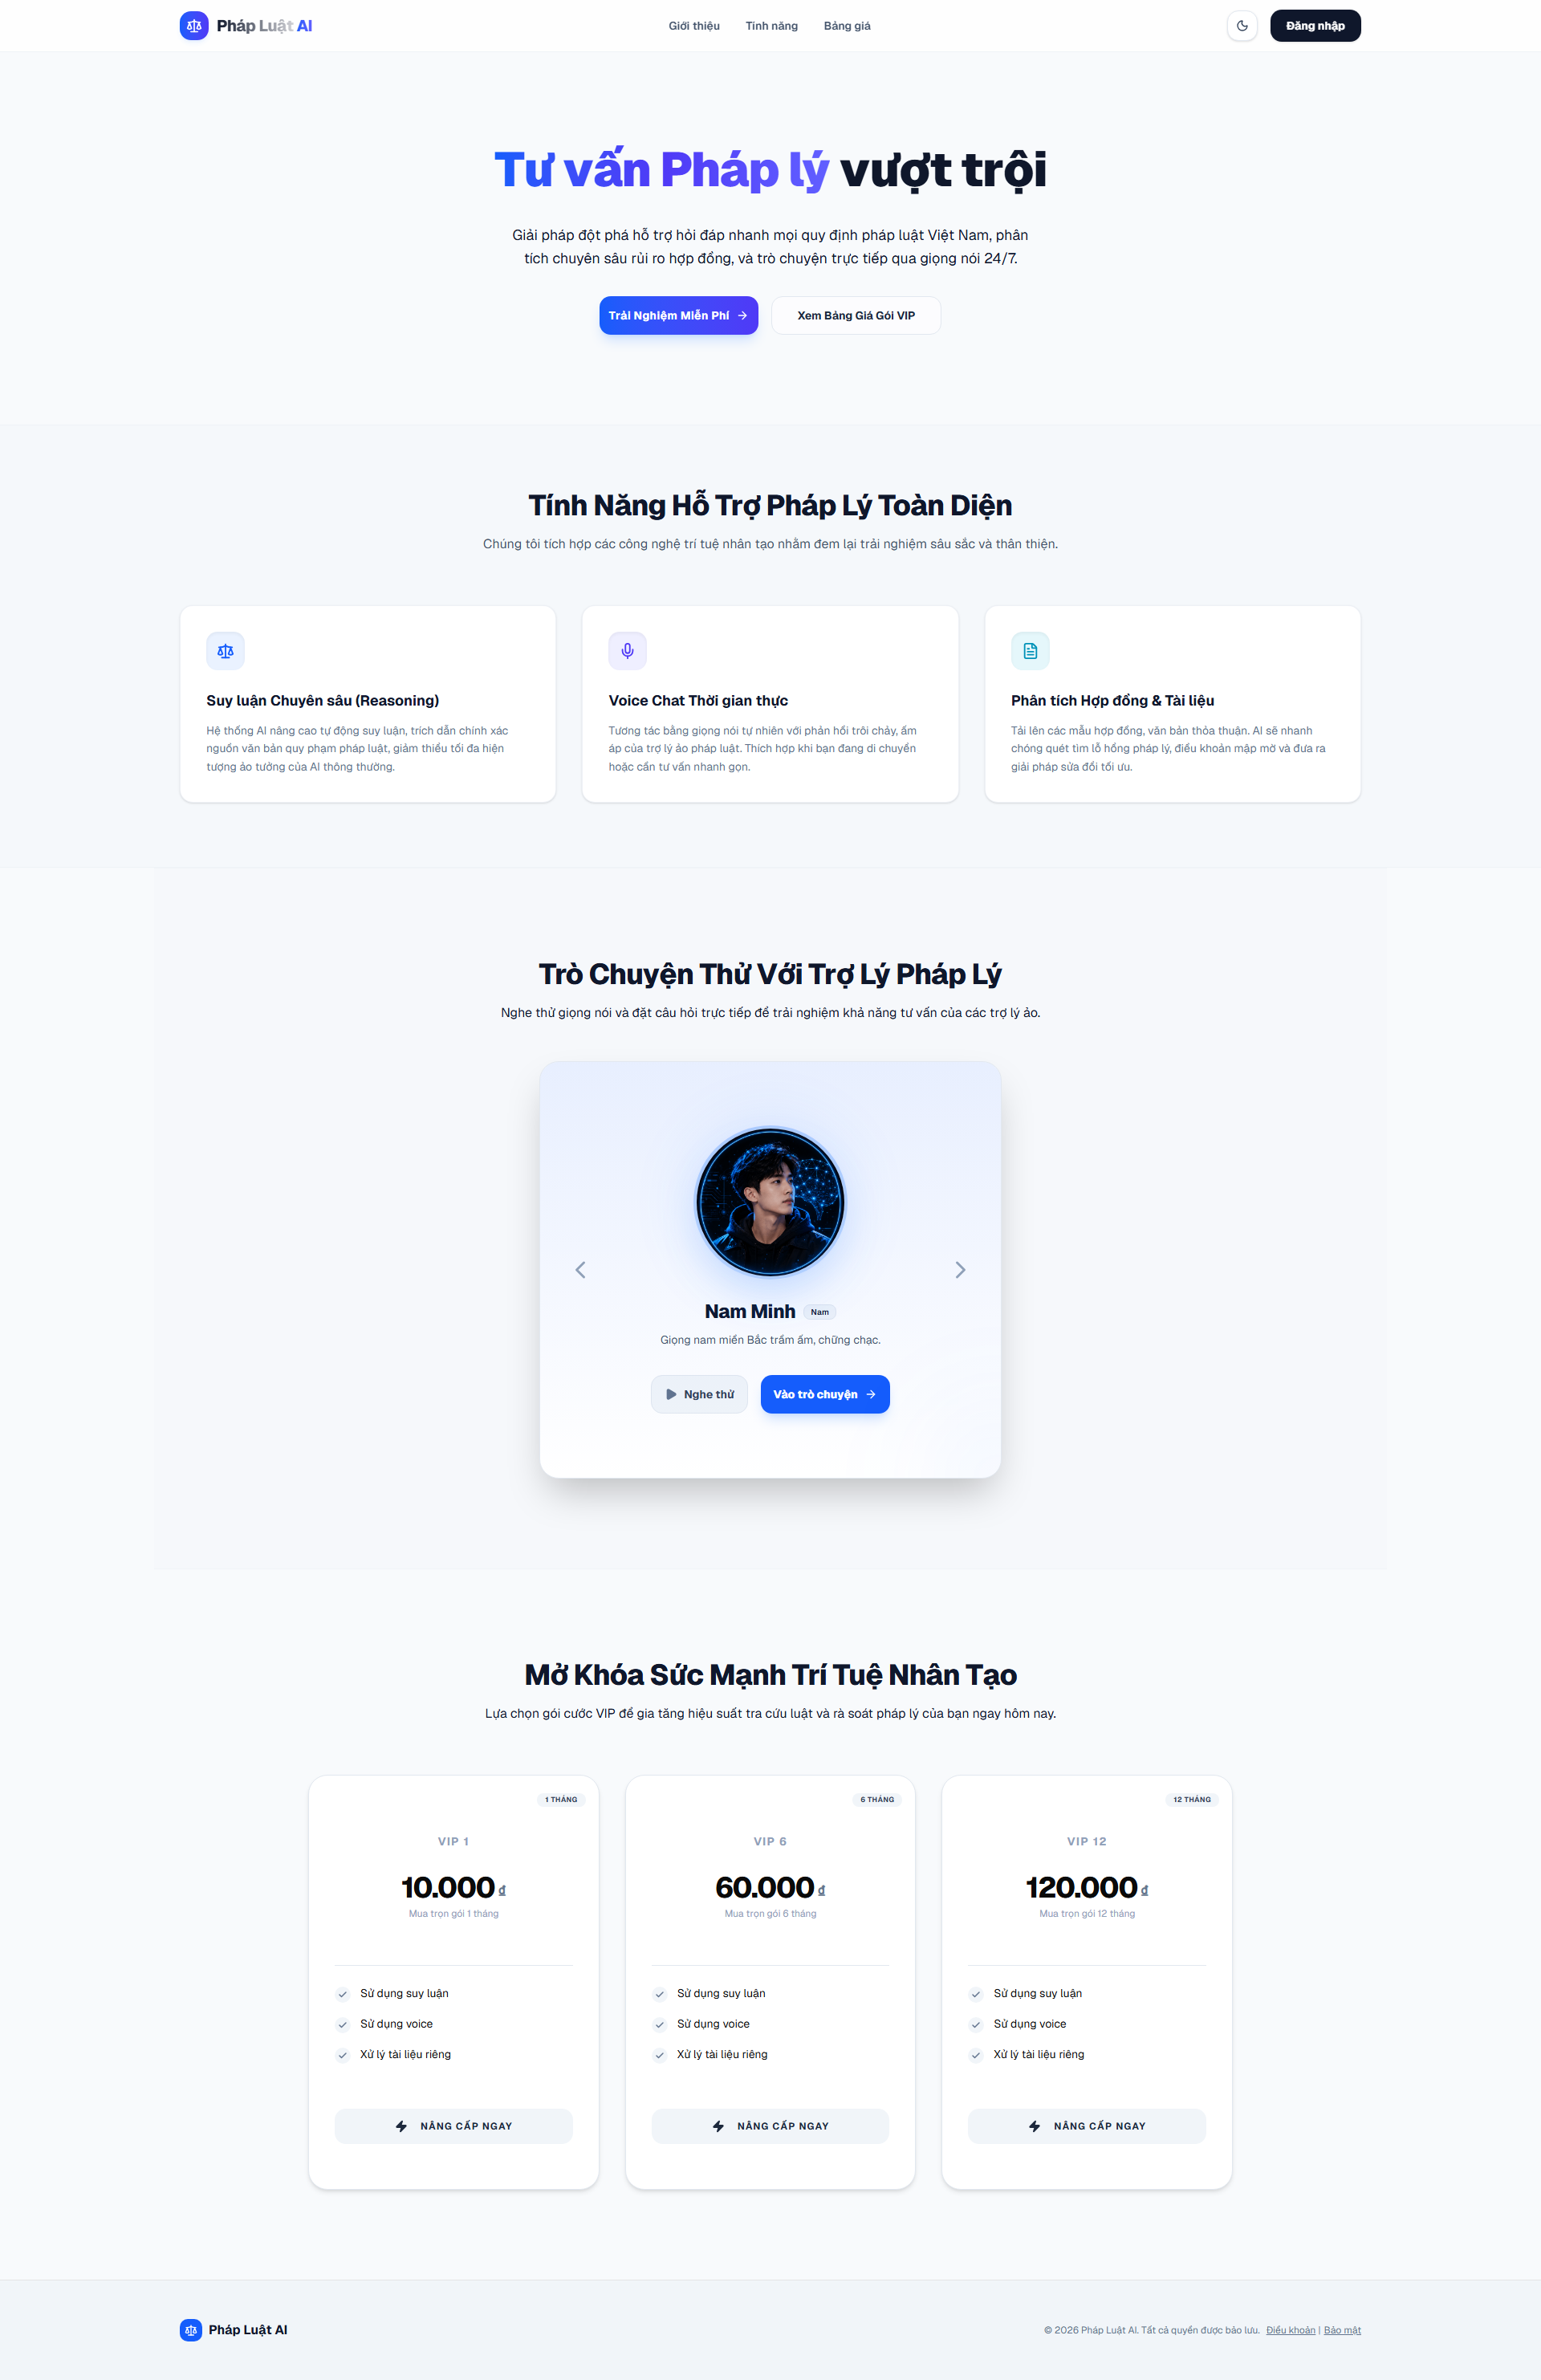
\includegraphics[width=0.92\textwidth]{images/WebUI-GuestHome.png}
\caption{Trang chủ khách}
\end{figure}

\textbf{Hướng dẫn:}

\begin{enumerate}
\item Người dùng truy cập trang chủ.
\item Xem phần giới thiệu, gói VIP và danh sách nhân vật.
\item Chọn đăng nhập hoặc đăng ký để bắt đầu sử dụng hệ thống.
\end{enumerate}




\subsubsection{Đăng ký tài khoản}

\begin{figure}[H]
\centering
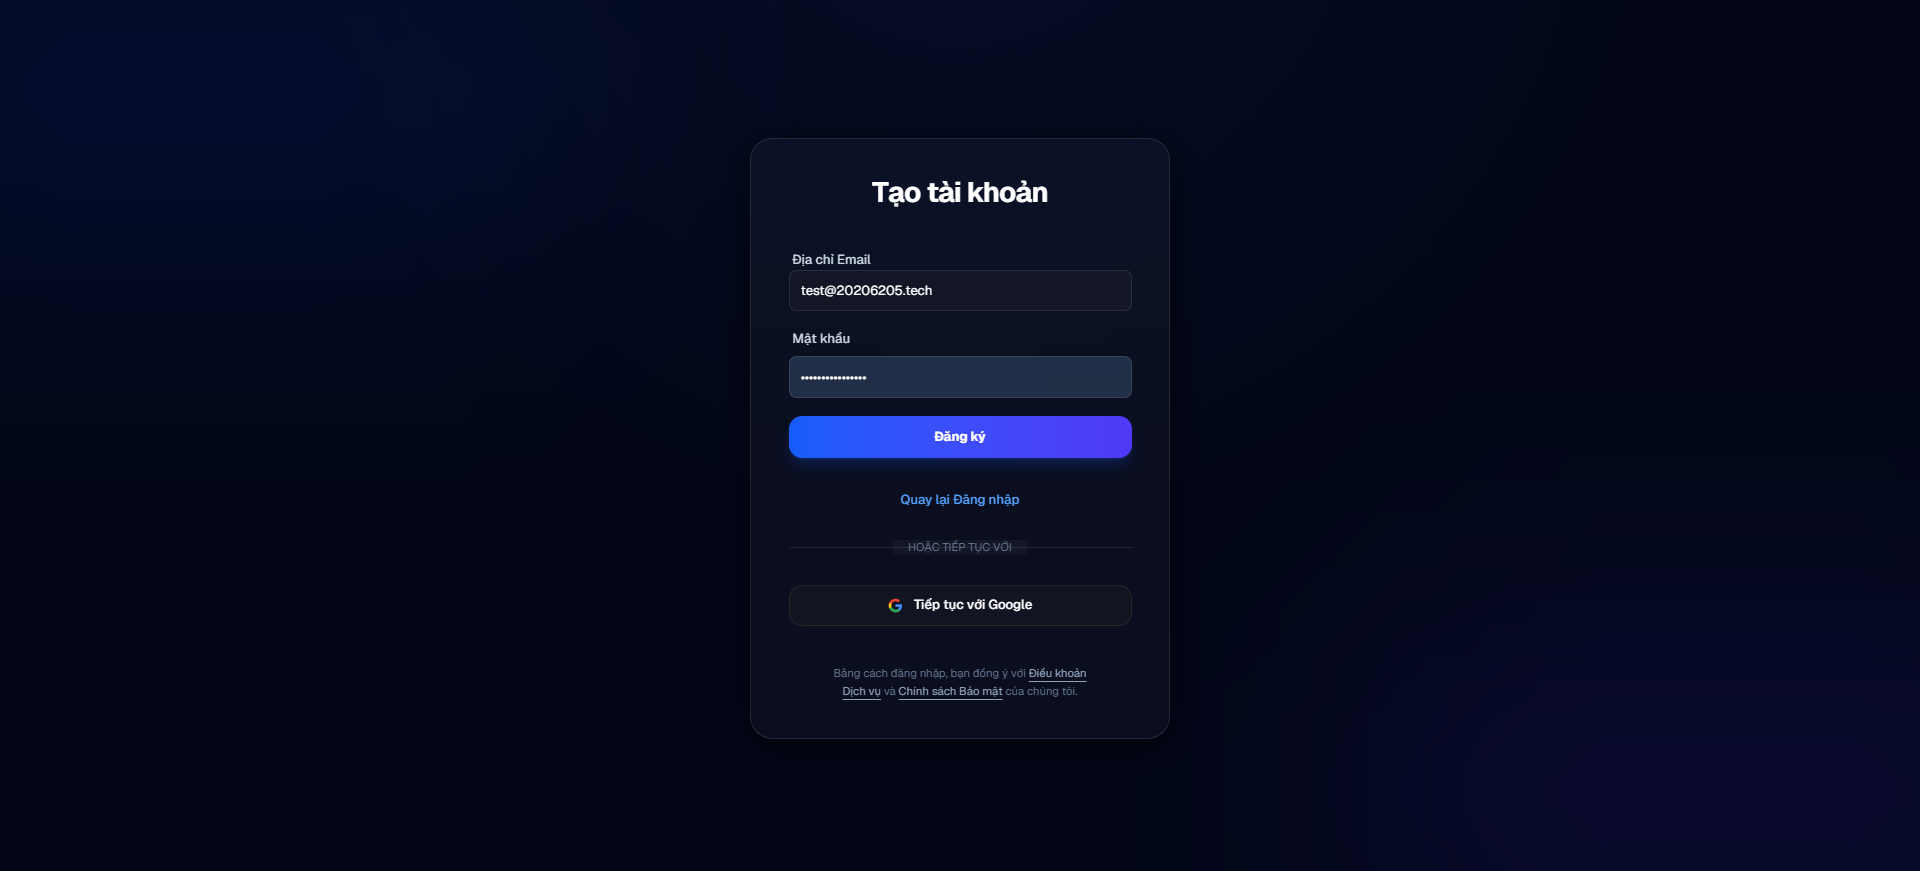
\includegraphics[width=0.92\textwidth]{images/WebUI-GuestRegister.png}
\caption{Đăng ký tài khoản}
\end{figure}

\textbf{Hướng dẫn:}

\begin{enumerate}
\item Nhập email và mật khẩu.
\item Bấm nút đăng ký.
\item Kiểm tra thông báo yêu cầu xác thực email.
\end{enumerate}

\subsubsection{Thông báo xác thực email}

\begin{figure}[H]
\centering
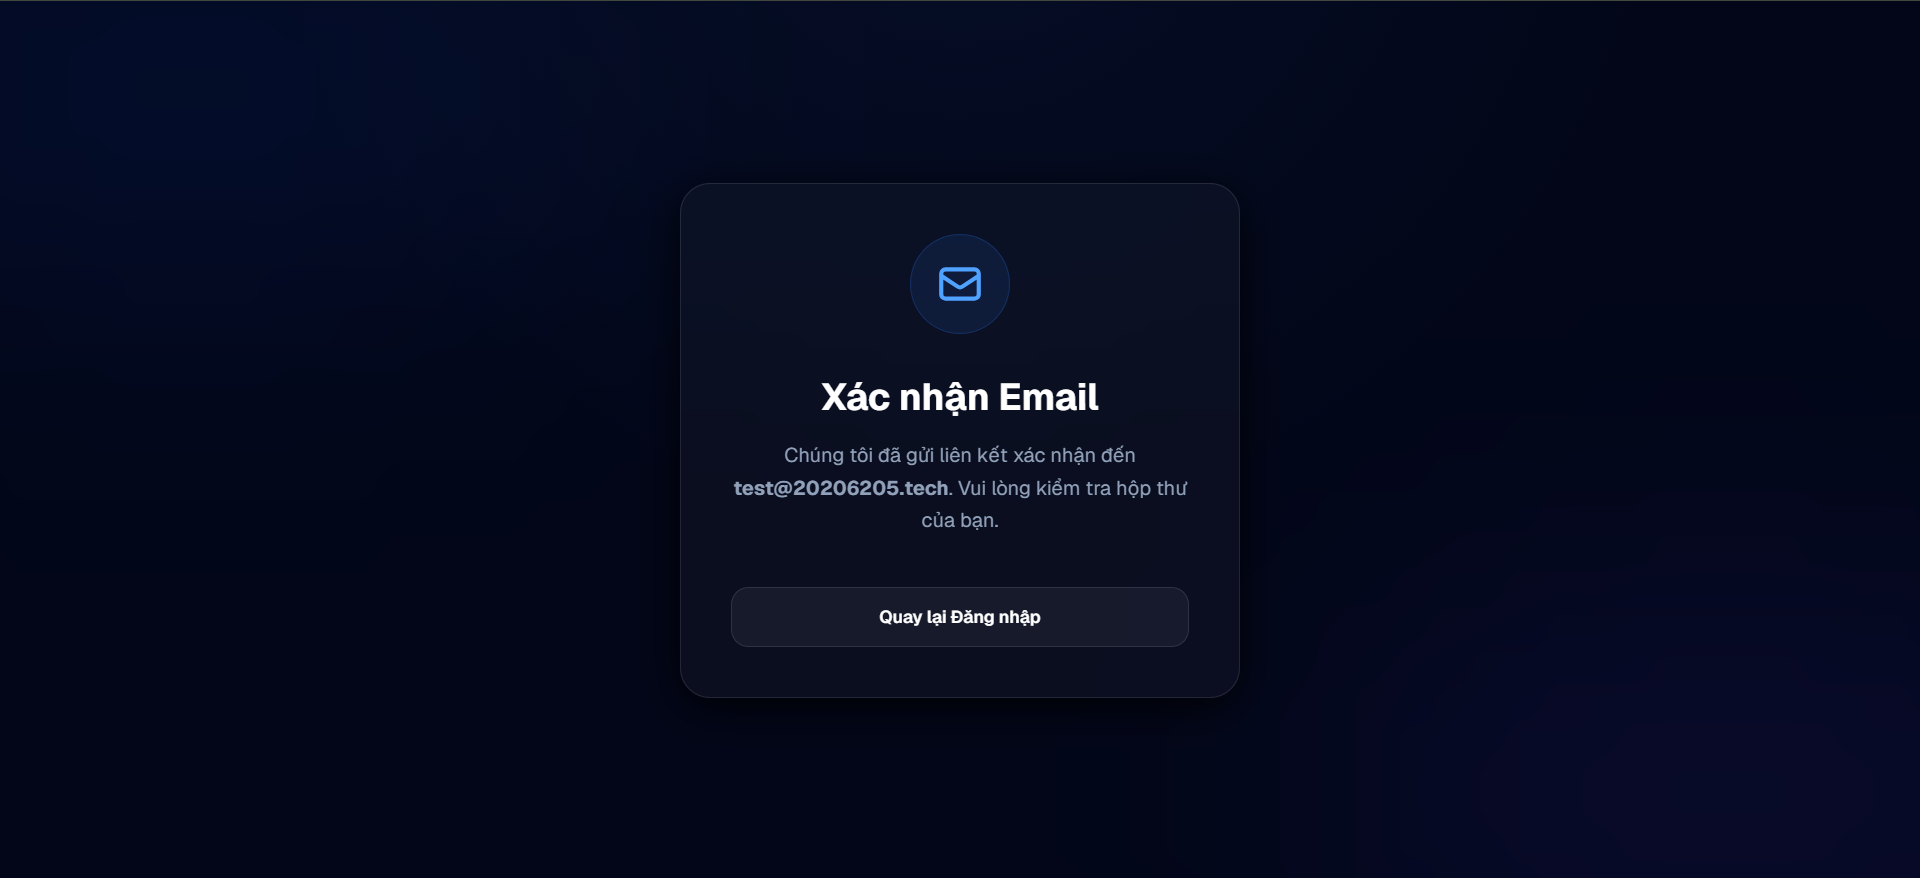
\includegraphics[width=0.92\textwidth]{images/WebUI-GuestSignupConfirmEmail.png}
\caption{Thông báo xác thực email}
\end{figure}

\textbf{Hướng dẫn:}

\begin{enumerate}
\item Sau khi đăng ký, hệ thống hiển thị trạng thái chờ xác thực.
\item Người dùng mở hộp thư email đã đăng ký.
\item Bấm liên kết xác thực để kích hoạt tài khoản.
\end{enumerate}

\subsubsection{Email xác thực đăng ký}

\begin{figure}[H]
\centering
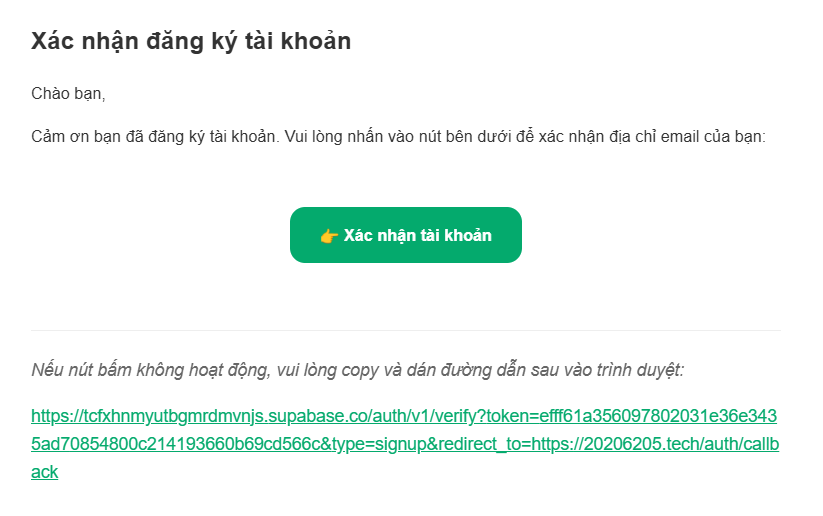
\includegraphics[width=0.92\textwidth]{images/WebUI-GuestRegistrationEmail.png}
\caption{Email xác thực đăng ký}
\end{figure}

\textbf{Hướng dẫn:}

\begin{enumerate}
\item Mở email xác thực từ hệ thống.
\item Kiểm tra đúng địa chỉ email và nội dung xác thực.
\item Bấm liên kết xác nhận để quay lại hệ thống.
\end{enumerate}

\subsubsection{Đăng nhập}

\begin{figure}[H]
\centering
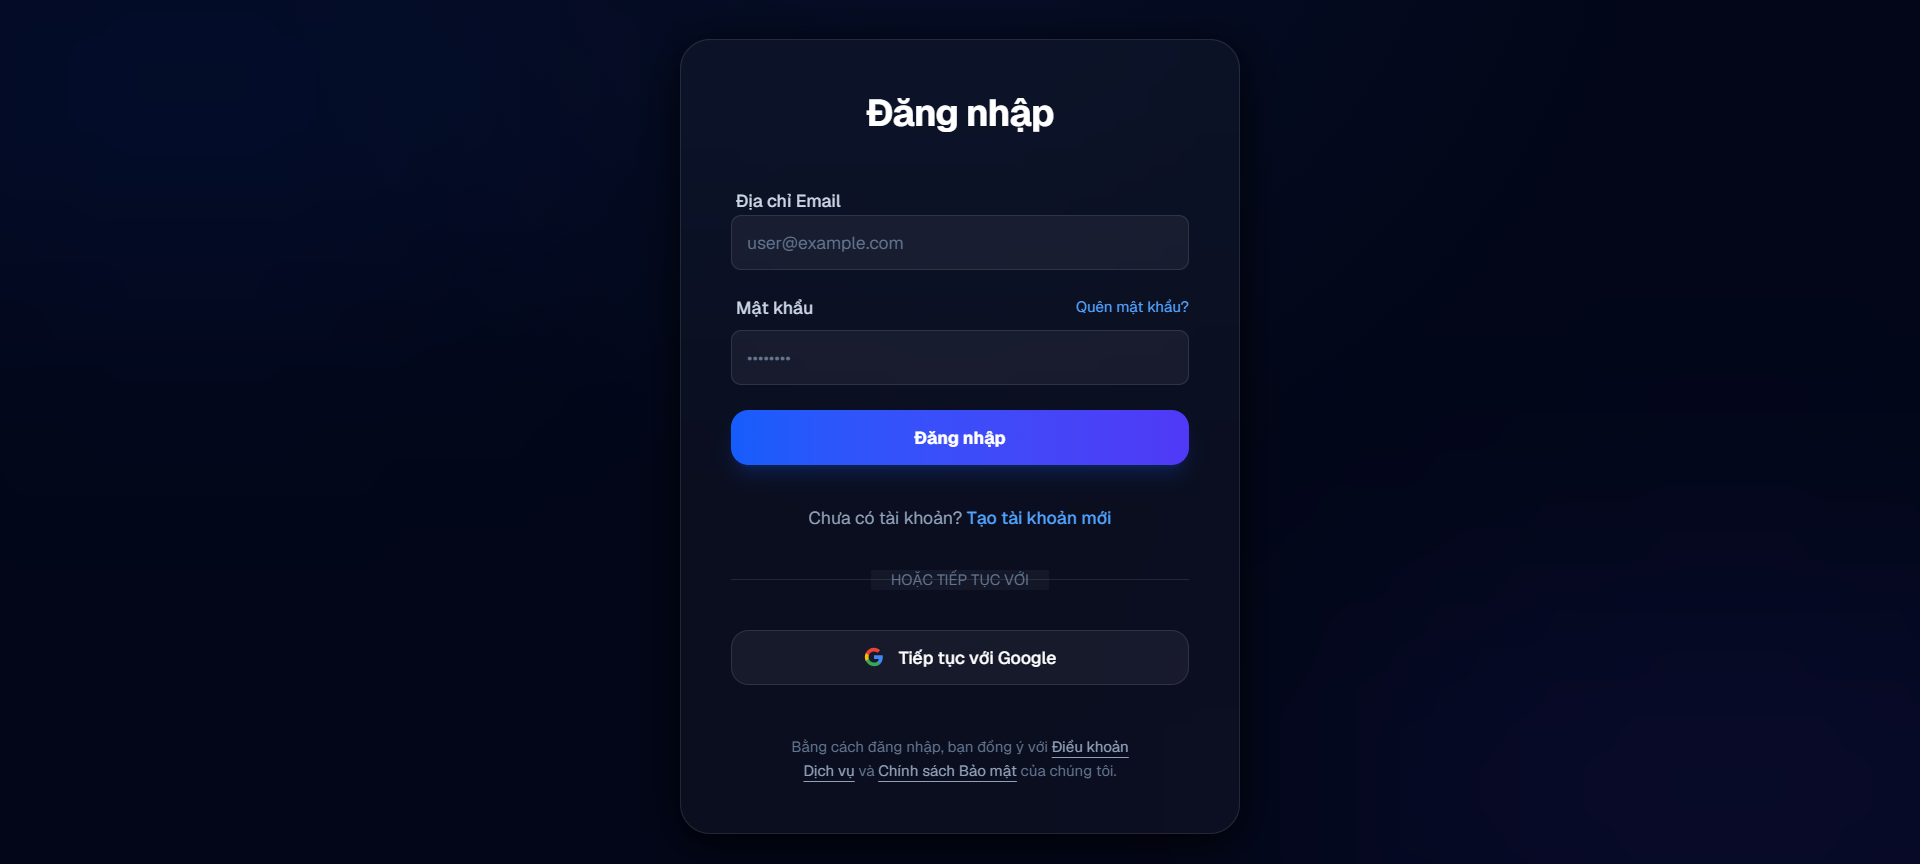
\includegraphics[width=0.92\textwidth]{images/WebUI-GuestLogin.png}
\caption{Đăng nhập}
\end{figure}

\textbf{Hướng dẫn:}

\begin{enumerate}
\item Nhập email và mật khẩu.
\item Bấm đăng nhập.
\item Nếu tài khoản bật MFA, hệ thống chuyển sang bước xác thực bổ sung.
\end{enumerate}

\subsubsection{Thiết lập MFA bằng mã QR}

\begin{figure}[H]
\centering
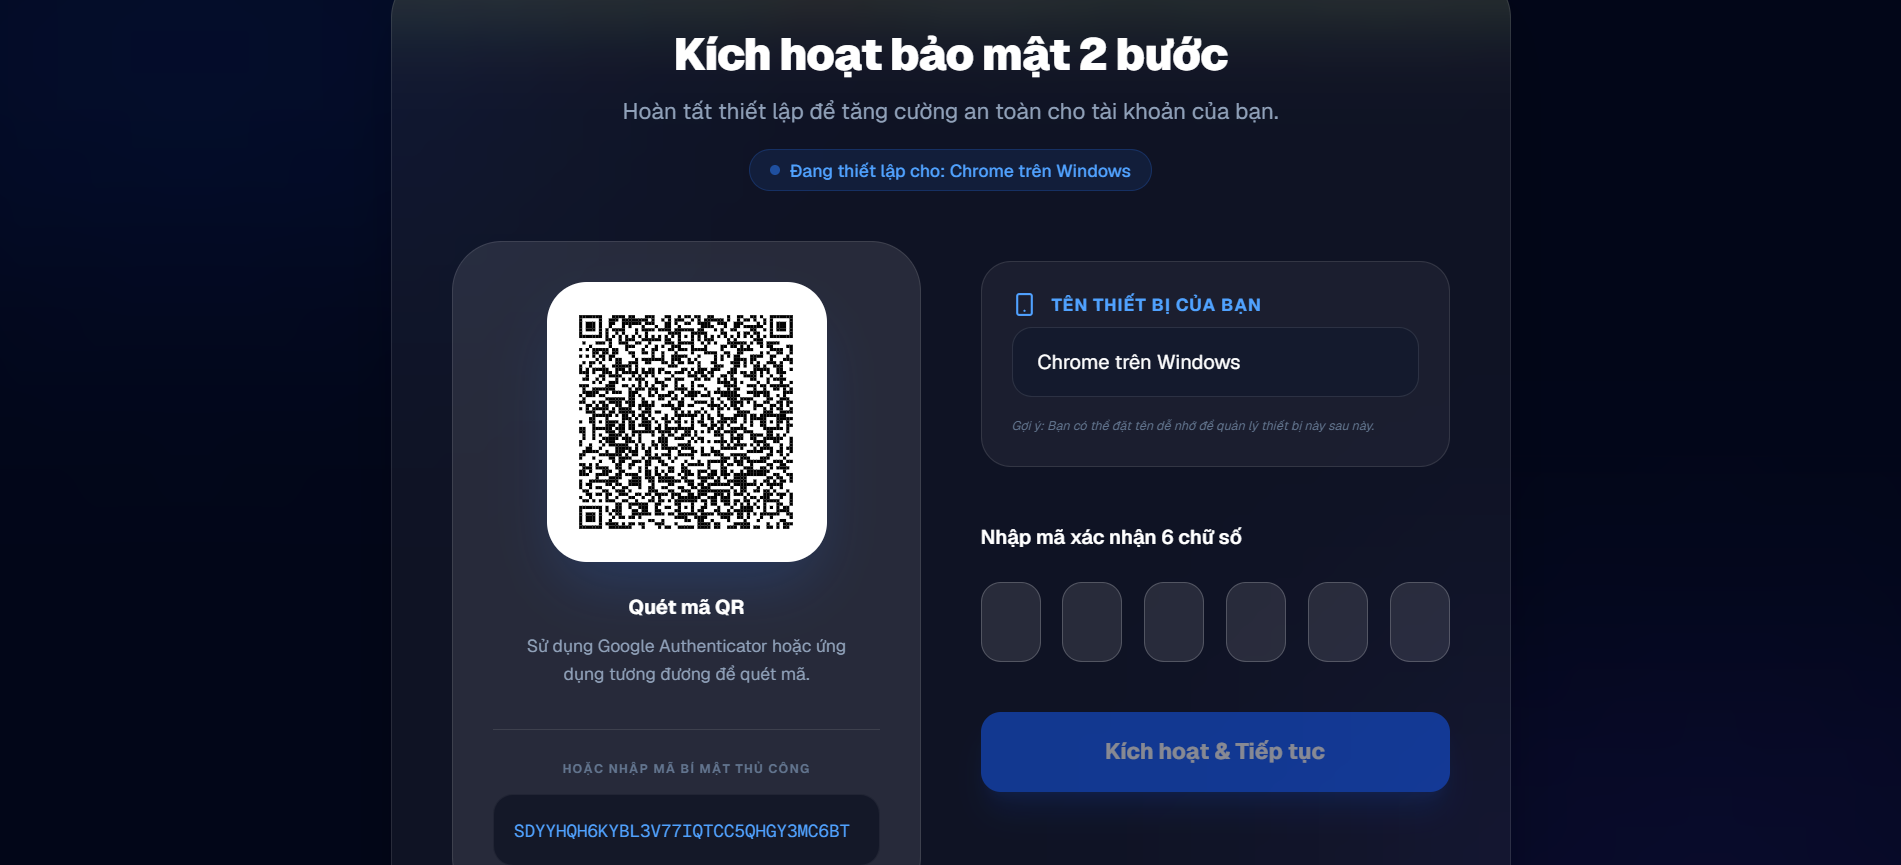
\includegraphics[width=0.92\textwidth]{images/WebUI-MfaQrSetup.png}
\caption{Thiết lập MFA bằng mã QR}
\end{figure}

\textbf{Hướng dẫn:}

\begin{enumerate}
\item Mở ứng dụng xác thực trên điện thoại.
\item Quét mã QR hiển thị trên màn hình.
\item Lưu cấu hình MFA trong ứng dụng xác thực.
\end{enumerate}

\subsubsection{Xác minh mã MFA}

\begin{figure}[H]
\centering
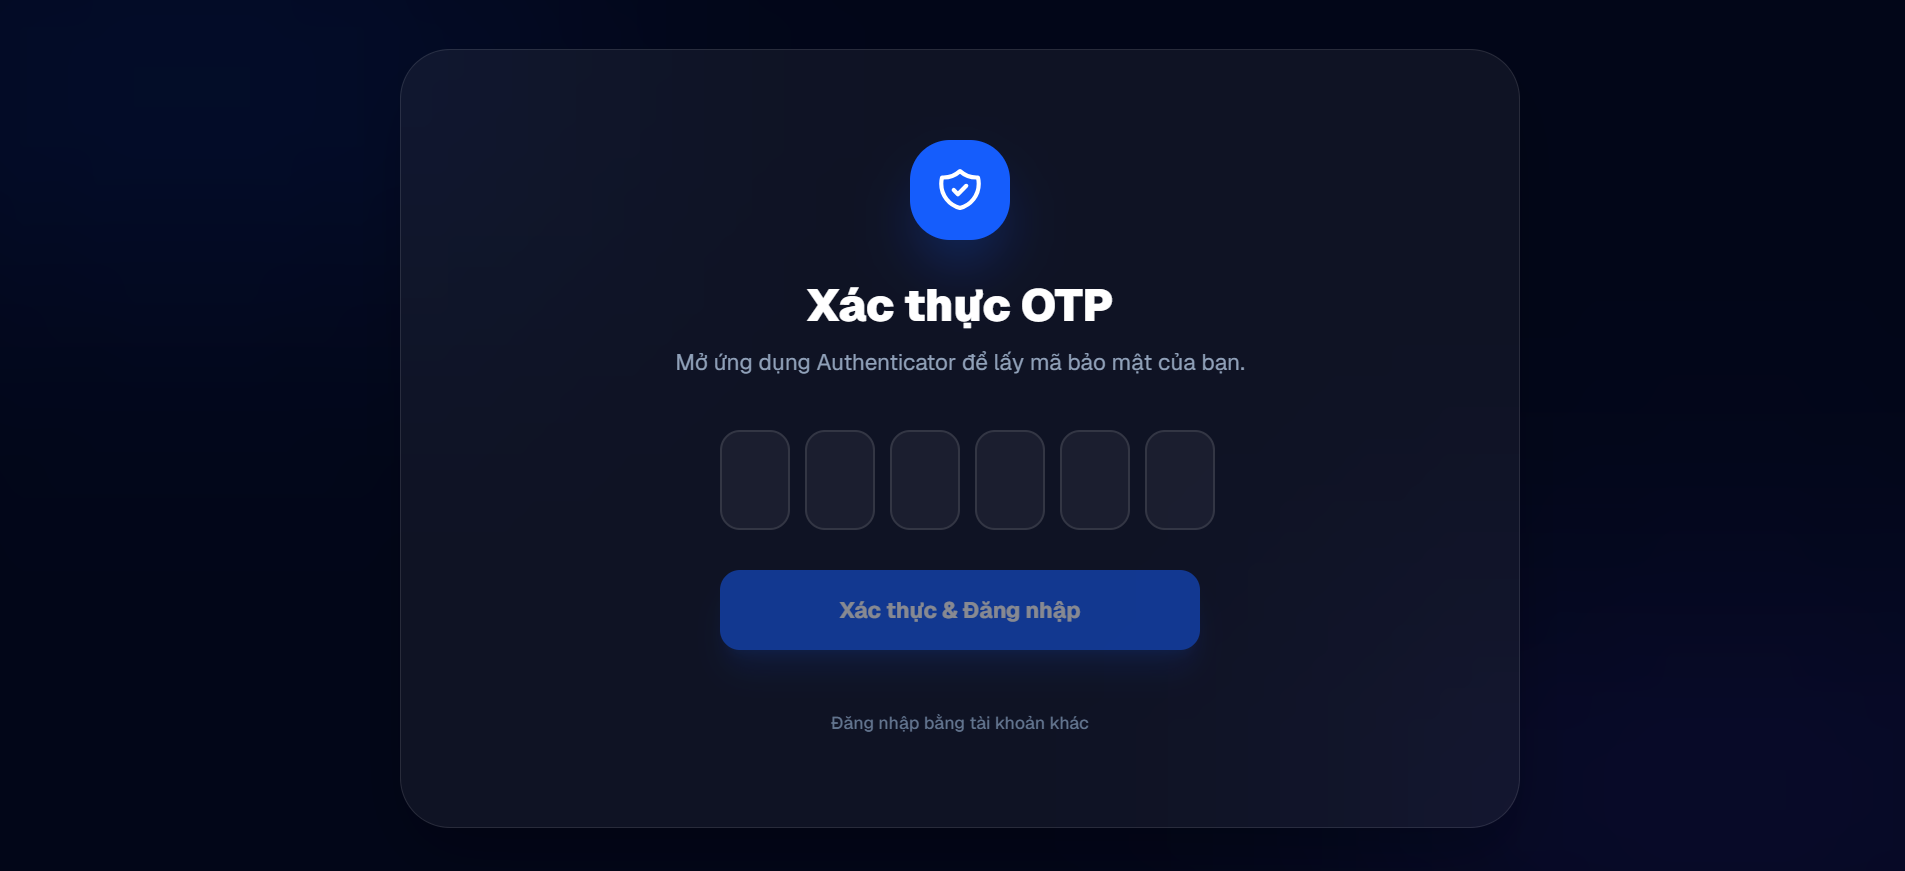
\includegraphics[width=0.92\textwidth]{images/WebUI-MfaCodeVerify.png}
\caption{Xác minh mã MFA}
\end{figure}

\textbf{Hướng dẫn:}

\begin{enumerate}
\item Lấy mã OTP mới nhất từ ứng dụng xác thực.
\item Nhập mã OTP vào màn hình xác minh.
\item Bấm xác nhận để hoàn tất đăng nhập hoặc kích hoạt MFA.
\end{enumerate}

\subsubsection{Hồ sơ người dùng}

\begin{figure}[H]
\centering
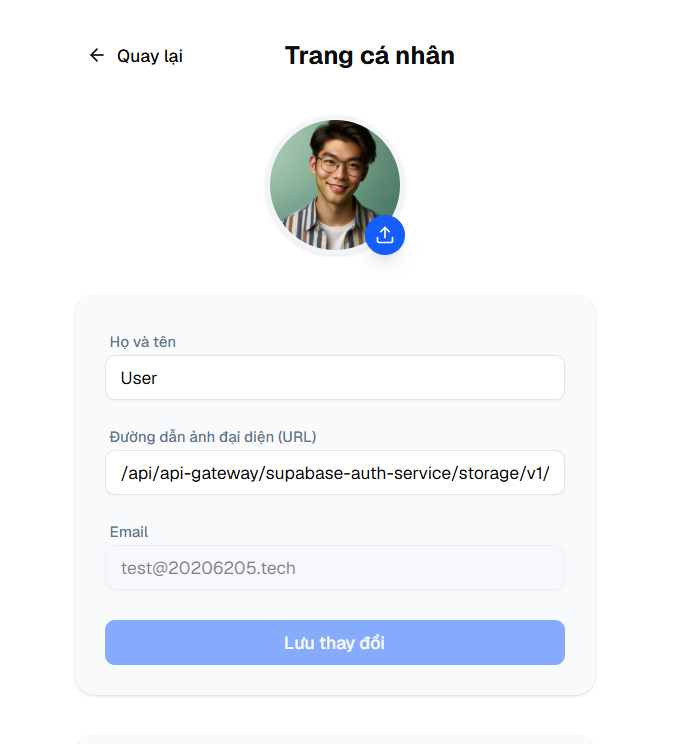
\includegraphics[width=0.92\textwidth]{images/WebUI-UserProfile.png}
\caption{Hồ sơ người dùng}
\end{figure}

\textbf{Hướng dẫn:}

\begin{enumerate}
\item Mở trang hồ sơ cá nhân.
\item Xem hoặc cập nhật thông tin hiển thị.
\item Lưu thay đổi để hệ thống cập nhật hồ sơ.
\end{enumerate}

\subsubsection{Đổi mật khẩu và MFA}

\begin{figure}[H]
\centering
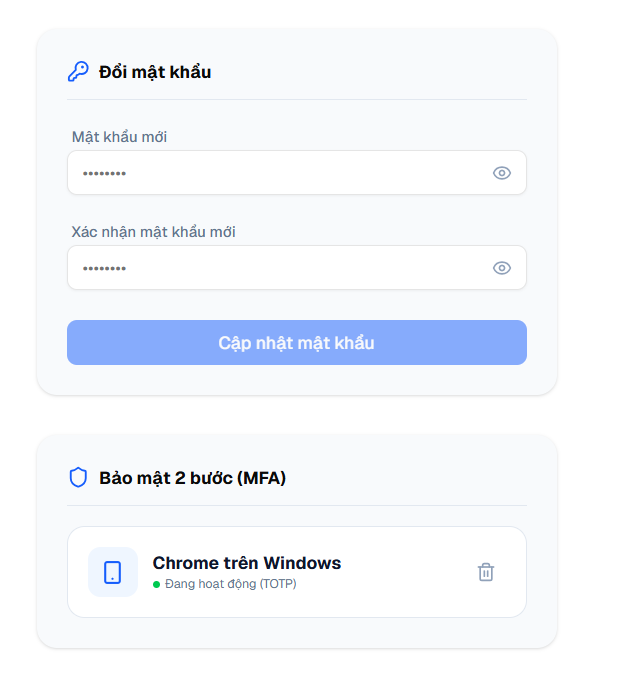
\includegraphics[width=0.92\textwidth]{images/WebUI-ChangePasswordAndMfa.png}
\caption{Đổi mật khẩu và MFA}
\end{figure}

\textbf{Hướng dẫn:}

\begin{enumerate}
\item Mở phần bảo mật tài khoản.
\item Đổi mật khẩu hoặc quản lý xác thực MFA.
\item Xác nhận thao tác theo yêu cầu của hệ thống.
\end{enumerate}

\subsubsection{Cài đặt người dùng}

\begin{figure}[H]
\centering
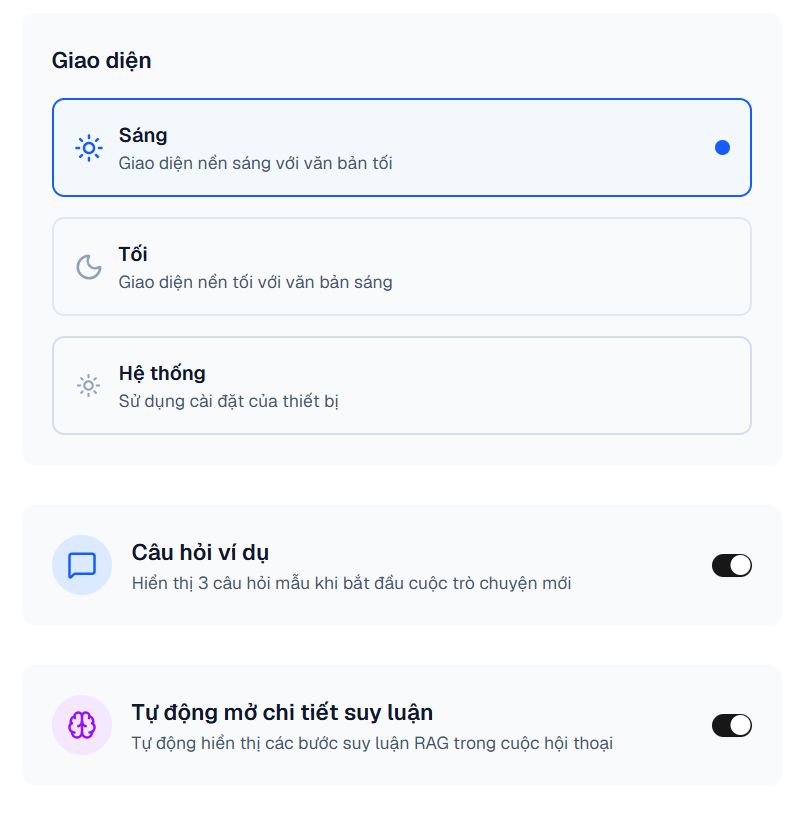
\includegraphics[width=0.92\textwidth]{images/WebUI-UserSettings.png}
\caption{Cài đặt người dùng}
\end{figure}

\textbf{Hướng dẫn:}

\begin{enumerate}
\item Mở trang cài đặt.
\item Điều chỉnh các tùy chọn cá nhân như giao diện, giọng nói hoặc cấu hình chat.
\item Bấm lưu để áp dụng cấu hình.
\end{enumerate}

\subsubsection{Khôi phục mật khẩu}

\begin{figure}[H]
\centering
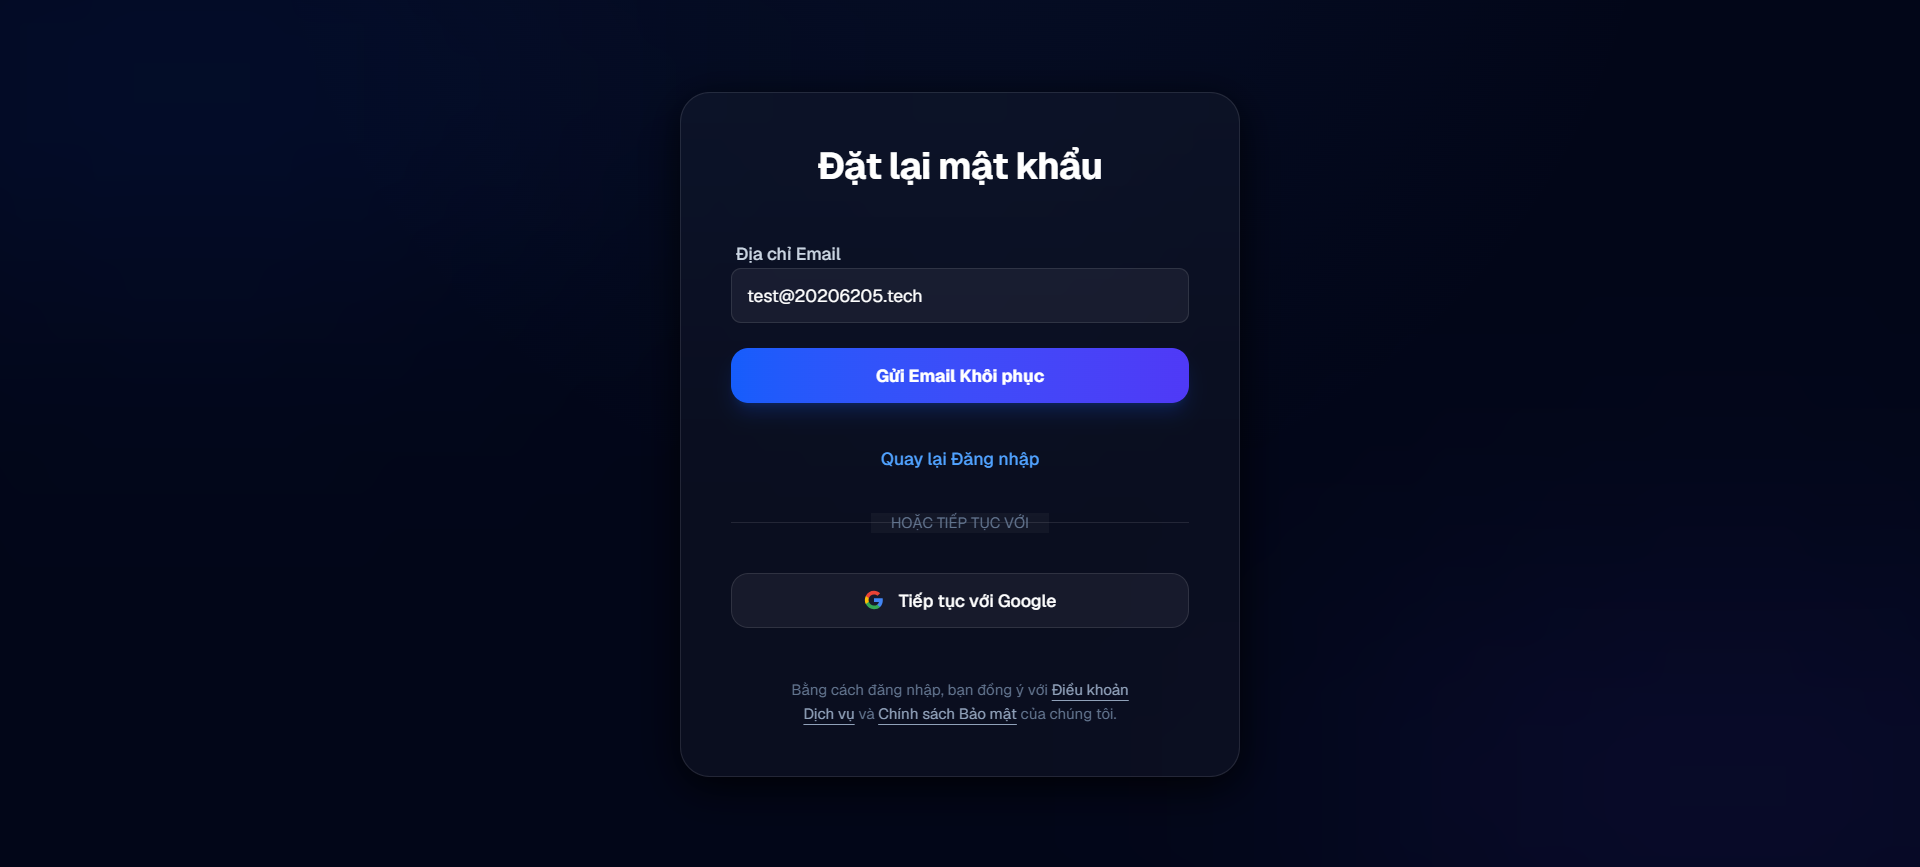
\includegraphics[width=0.92\textwidth]{images/WebUI-ResetPassword.png}
\caption{Khôi phục mật khẩu}
\end{figure}

\textbf{Hướng dẫn:}

\begin{enumerate}
\item Nhập email đã đăng ký.
\item Bấm gửi yêu cầu khôi phục.
\item Mở email khôi phục mật khẩu và làm theo hướng dẫn.
\end{enumerate}

\subsubsection{Email khôi phục mật khẩu}

\begin{figure}[H]
\centering
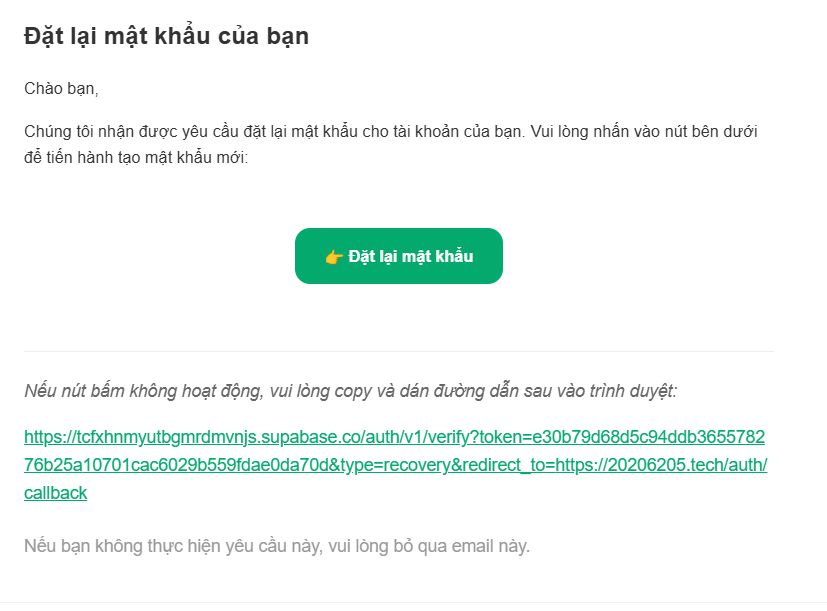
\includegraphics[width=0.92\textwidth]{images/WebUI-PasswordResetEmail.png}
\caption{Email khôi phục mật khẩu}
\end{figure}

\textbf{Hướng dẫn:}

\begin{enumerate}
\item Mở email khôi phục mật khẩu.
\item Bấm liên kết đặt lại mật khẩu.
\item Nhập mật khẩu mới trên màn hình được chuyển hướng.
\end{enumerate}

\subsection{2. Trò chuyện, ghi chú và chia sẻ}

\subsubsection{Chat văn bản}

\begin{figure}[H]
\centering
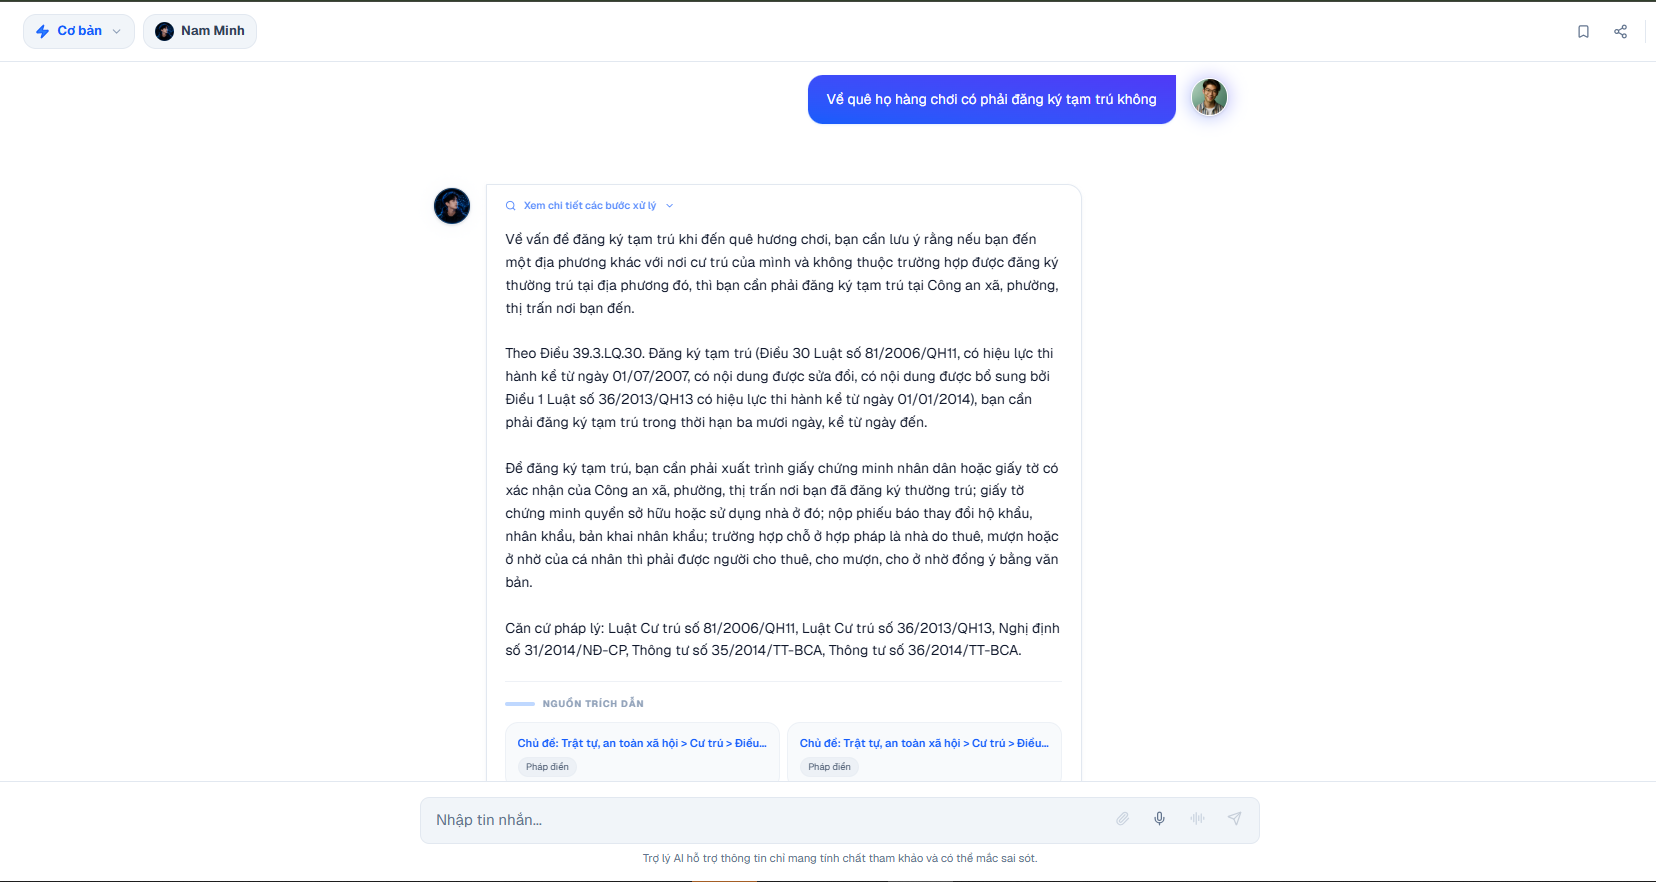
\includegraphics[width=0.92\textwidth]{images/WebUI-ChatText.png}
\caption{Chat văn bản}
\end{figure}

\textbf{Hướng dẫn:}

\begin{enumerate}
\item Nhập câu hỏi vào khung chat.
\item Chọn tùy chọn bổ sung nếu cần, ví dụ reasoning hoặc tài liệu đính kèm.
\item Gửi câu hỏi và theo dõi phản hồi dạng streaming.
\end{enumerate}

\subsubsection{Chat bằng micro}

\begin{figure}[H]
\centering
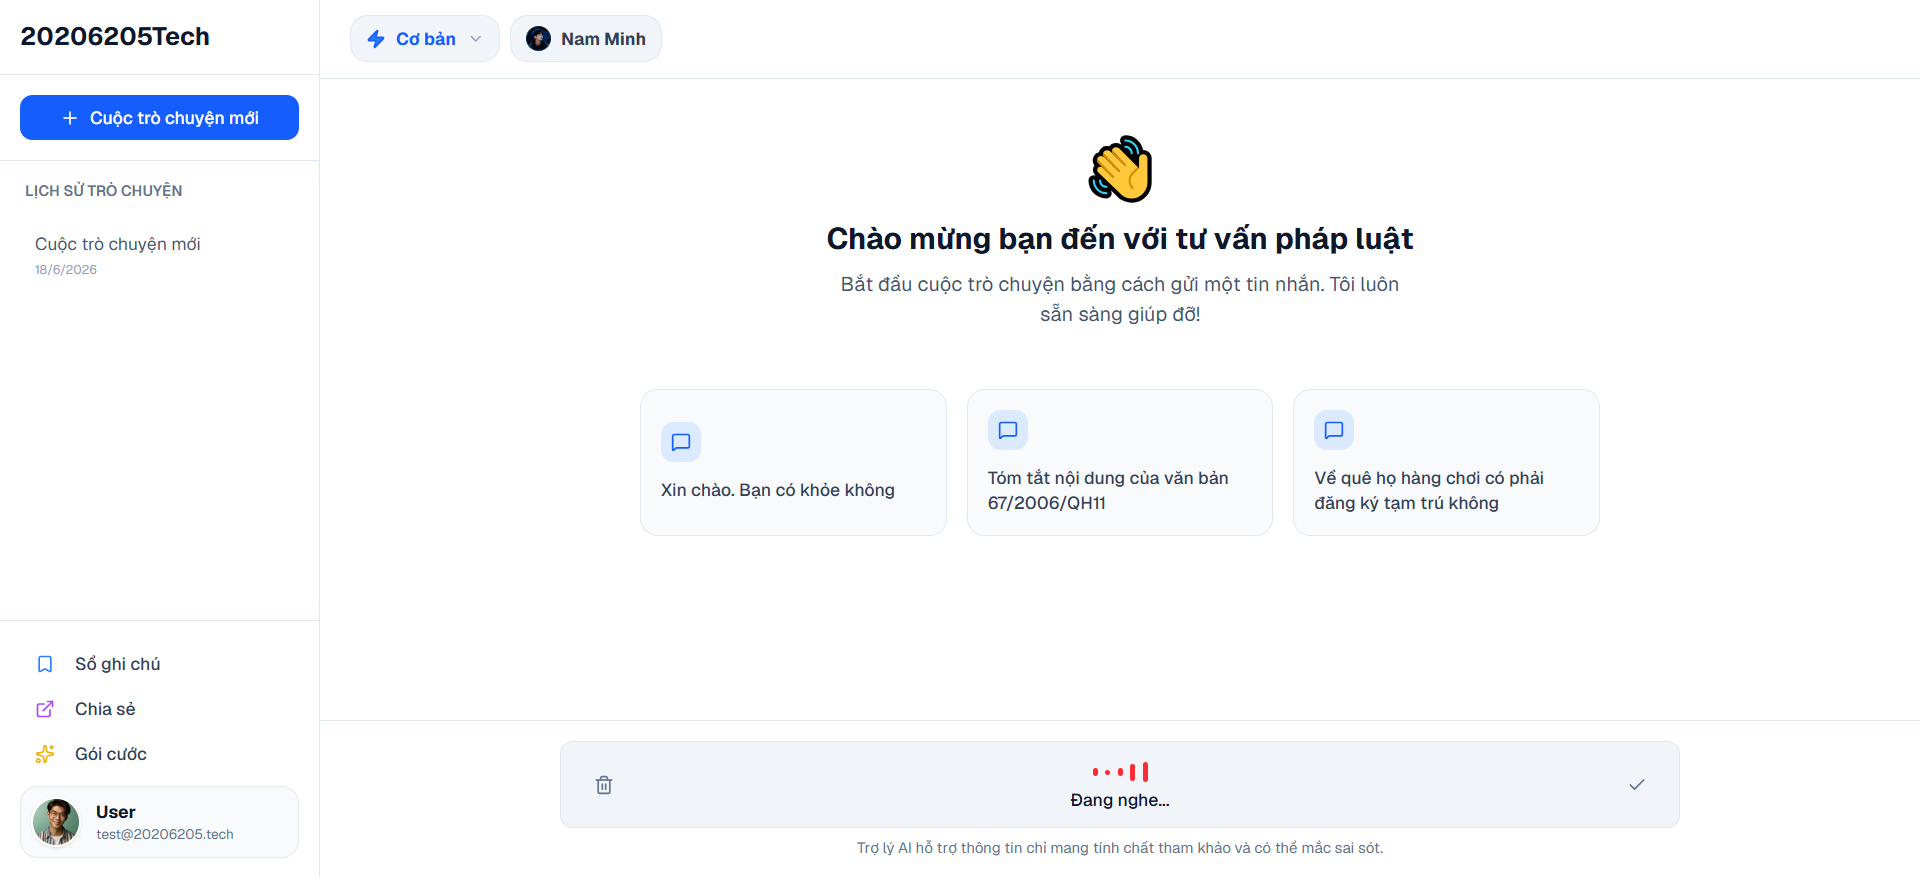
\includegraphics[width=0.92\textwidth]{images/WebUI-ChatMicrophone.png}
\caption{Chat bằng micro}
\end{figure}

\textbf{Hướng dẫn:}

\begin{enumerate}
\item Bấm biểu tượng micro để bắt đầu nhập bằng giọng nói.
\item Cho phép trình duyệt truy cập micro nếu được hỏi.
\item Nói câu hỏi và chờ hệ thống xử lý.
\end{enumerate}

\subsubsection{Tạo ghi chú bookmark}

\begin{figure}[H]
\centering
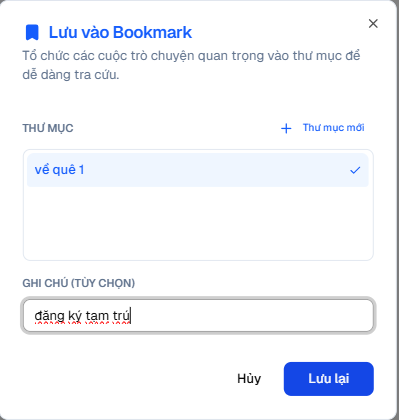
\includegraphics[width=0.92\textwidth]{images/WebUI-BookmarkNoteCreate.png}
\caption{Tạo ghi chú bookmark}
\end{figure}

\textbf{Hướng dẫn:}

\begin{enumerate}
\item Chọn cuộc hội thoại cần lưu.
\item Chọn hoặc tạo thư mục bookmark.
\item Nhập ghi chú và bấm lưu.
\end{enumerate}

\subsubsection{Quản lý ghi chú bookmark}

\begin{figure}[H]
\centering
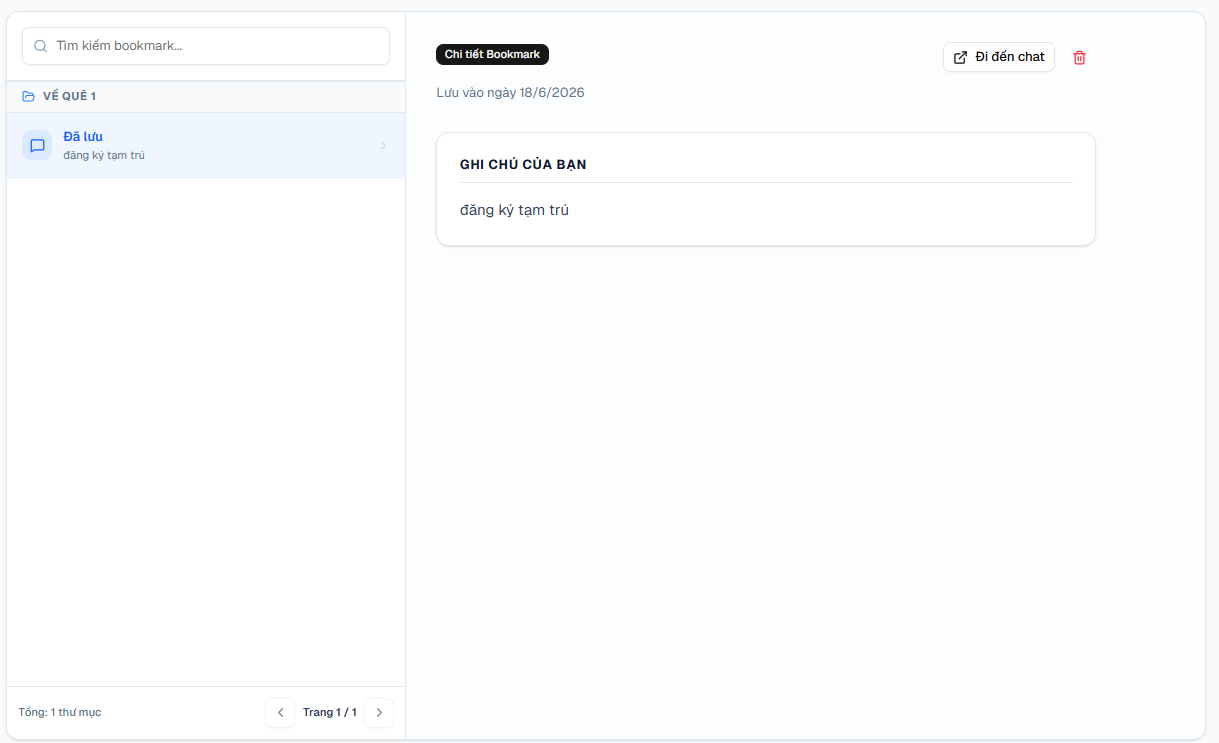
\includegraphics[width=0.92\textwidth]{images/WebUI-BookmarkNoteManage.png}
\caption{Quản lý ghi chú bookmark}
\end{figure}

\textbf{Hướng dẫn:}

\begin{enumerate}
\item Mở danh sách bookmark.
\item Tìm cuộc hội thoại hoặc thư mục cần quản lý.
\item Chỉnh sửa ghi chú, đổi thư mục hoặc mở lại cuộc hội thoại.
\end{enumerate}

\subsubsection{Tạo liên kết chia sẻ}

\begin{figure}[H]
\centering
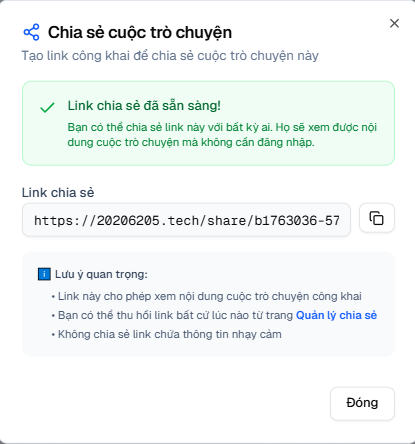
\includegraphics[width=0.92\textwidth]{images/WebUI-ShareCreate.png}
\caption{Tạo liên kết chia sẻ}
\end{figure}

\textbf{Hướng dẫn:}

\begin{enumerate}
\item Mở cuộc hội thoại cần chia sẻ.
\item Bấm tạo liên kết chia sẻ.
\item Sao chép liên kết sau khi hệ thống tạo xong.
\end{enumerate}

\subsubsection{Quản lý chia sẻ}

\begin{figure}[H]
\centering
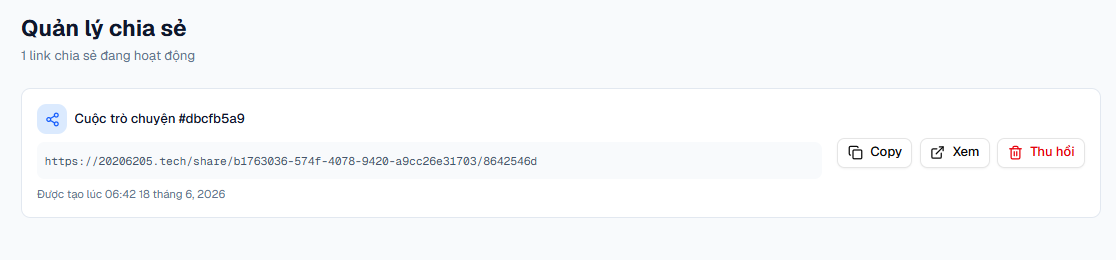
\includegraphics[width=0.92\textwidth]{images/WebUI-ShareManage.png}
\caption{Quản lý chia sẻ}
\end{figure}

\textbf{Hướng dẫn:}

\begin{enumerate}
\item Mở danh sách liên kết chia sẻ.
\item Kiểm tra trạng thái từng liên kết.
\item Thu hồi liên kết nếu không muốn tiếp tục chia sẻ.
\end{enumerate}

\subsubsection{Liên kết chia sẻ không khả dụng}

\begin{figure}[H]
\centering
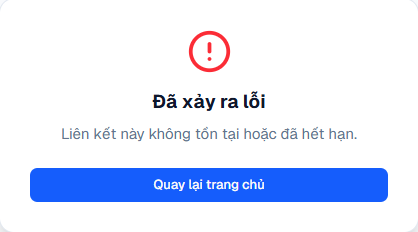
\includegraphics[width=0.92\textwidth]{images/WebUI-ShareLinkUnavailable.png}
\caption{Liên kết chia sẻ không khả dụng}
\end{figure}

\textbf{Hướng dẫn:}

\begin{enumerate}
\item Người nhận mở liên kết chia sẻ.
\item Nếu liên kết đã bị thu hồi hoặc không tồn tại, hệ thống hiển thị thông báo không khả dụng.
\item Liên hệ người chia sẻ để nhận liên kết mới nếu cần.
\end{enumerate}

\subsubsection{Liên kết chia sẻ khả dụng}

\begin{figure}[H]
\centering
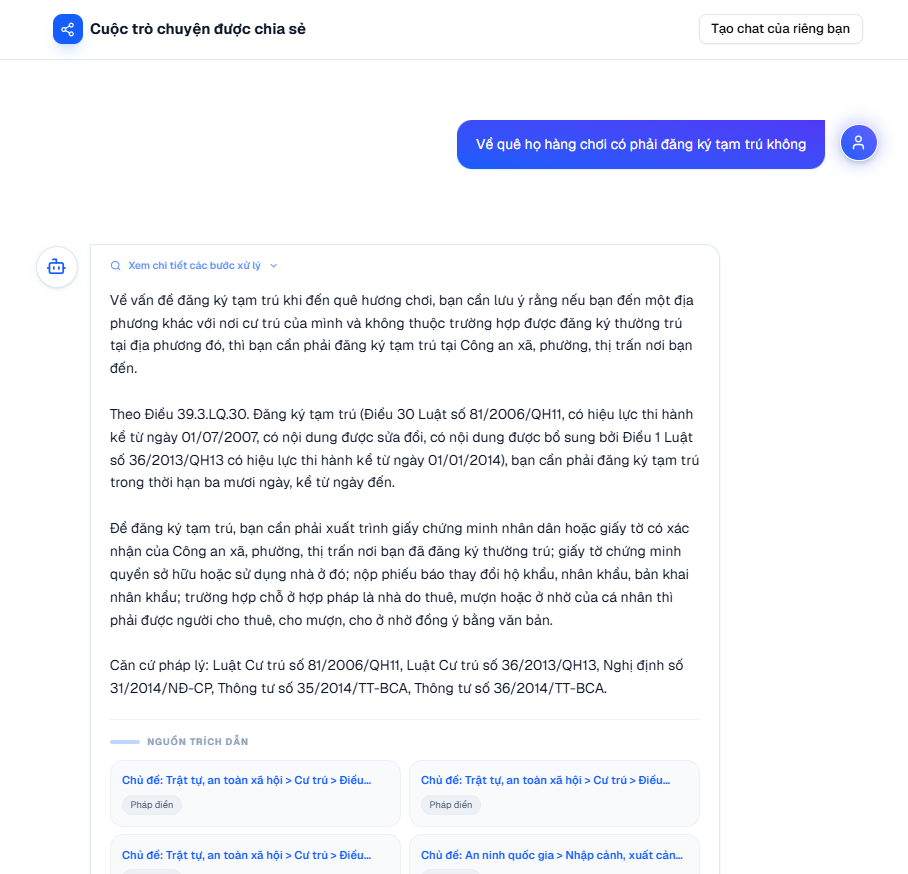
\includegraphics[width=0.92\textwidth]{images/WebUI-ShareLinkDone.png}
\caption{Liên kết chia sẻ khả dụng}
\end{figure}

\textbf{Hướng dẫn:}

\begin{enumerate}
\item Mở liên kết chia sẻ hợp lệ.
\item Xem nội dung hội thoại được chia sẻ.
\item Dùng nội dung này để tham khảo mà không cần quyền chỉnh sửa cuộc hội thoại gốc.
\end{enumerate}

\subsubsection{Thu hồi chia sẻ}

\begin{figure}[H]
\centering
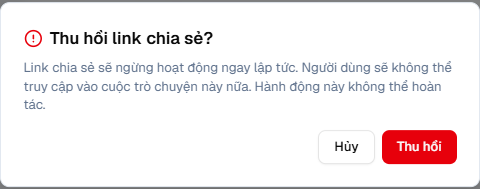
\includegraphics[width=0.92\textwidth]{images/WebUI-ShareRevoke.png}
\caption{Thu hồi chia sẻ}
\end{figure}

\textbf{Hướng dẫn:}

\begin{enumerate}
\item Chọn liên kết chia sẻ cần thu hồi.
\item Bấm thu hồi hoặc hủy chia sẻ.
\item Xác nhận thao tác để liên kết không còn truy cập được.
\end{enumerate}

\subsubsection{Xóa cuộc trò chuyện}

\begin{figure}[H]
\centering
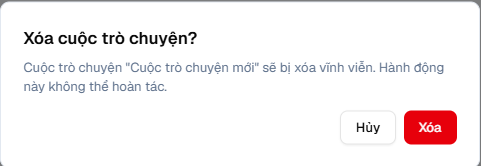
\includegraphics[width=0.92\textwidth]{images/WebUI-ChatDelete.png}
\caption{Xóa cuộc trò chuyện}
\end{figure}

\textbf{Hướng dẫn:}

\begin{enumerate}
\item Chọn cuộc trò chuyện cần xóa.
\item Bấm thao tác xóa.
\item Xác nhận để hệ thống xóa hoặc ẩn cuộc trò chuyện khỏi danh sách.
\end{enumerate}

\subsection{3. Quản trị hệ thống}

\subsubsection{Quản lý gói VIP}

\begin{figure}[H]
\centering
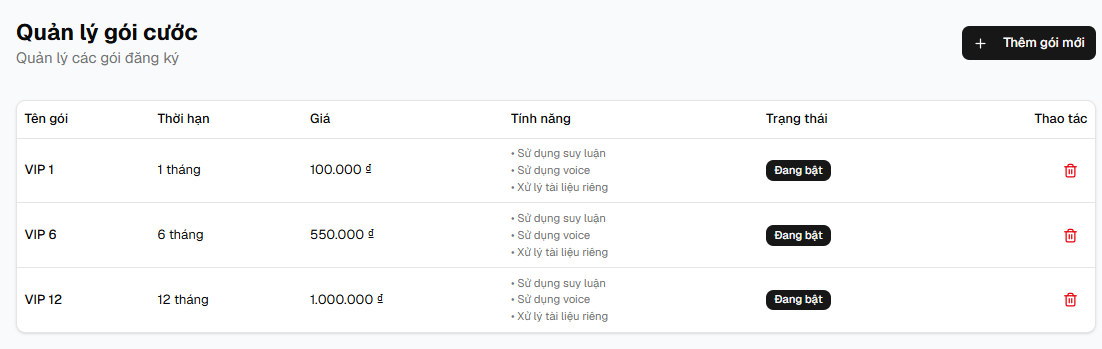
\includegraphics[width=0.92\textwidth]{images/WebUI-AdminPlans.png}
\caption{Quản lý gói VIP}
\end{figure}

\textbf{Hướng dẫn:}

\begin{enumerate}
\item Admin mở trang quản lý gói VIP.
\item Xem danh sách gói hiện có.
\item Tạo mới, cập nhật hoặc vô hiệu hóa gói theo nhu cầu.
\end{enumerate}

\subsubsection{Quản lý nhân vật}

\begin{figure}[H]
\centering
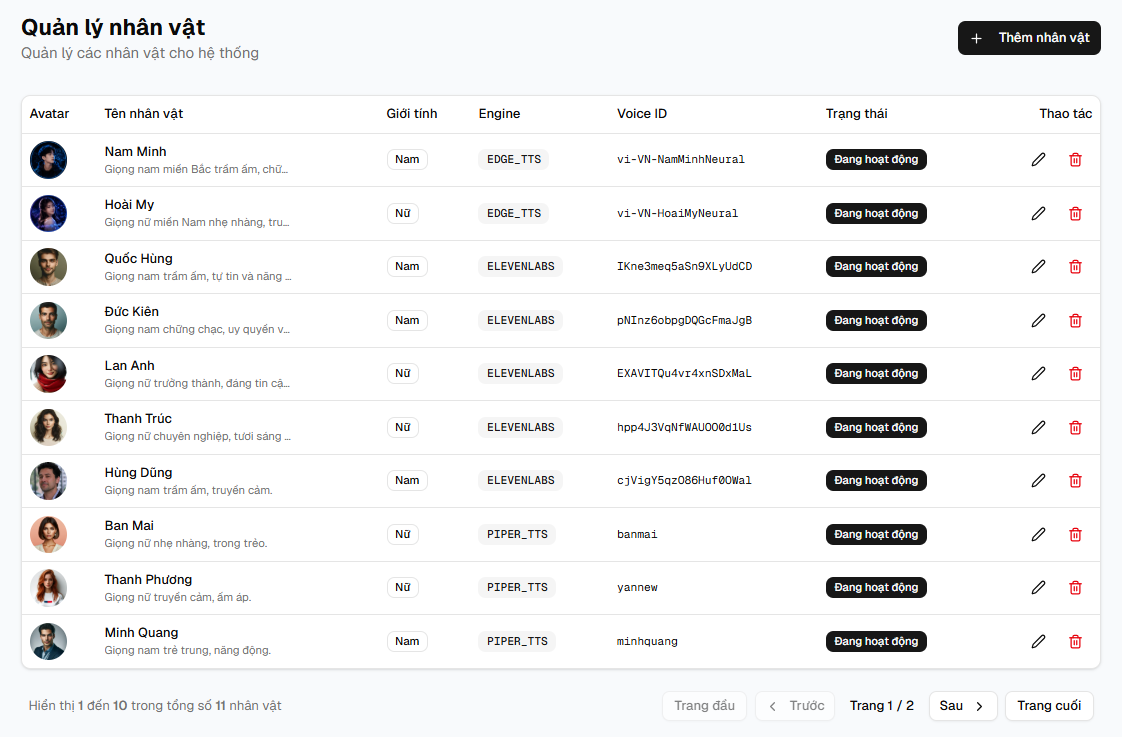
\includegraphics[width=0.92\textwidth]{images/WebUI-AdminPersonas.png}
\caption{Quản lý nhân vật}
\end{figure}

\textbf{Hướng dẫn:}

\begin{enumerate}
\item Admin mở trang quản lý nhân vật.
\item Nhập thông tin nhân vật, prompt, ảnh đại diện và giọng nói.
\item Lưu để nhân vật xuất hiện trong hệ thống.
\end{enumerate}

\subsubsection{Quản lý engine}

\begin{figure}[H]
\centering
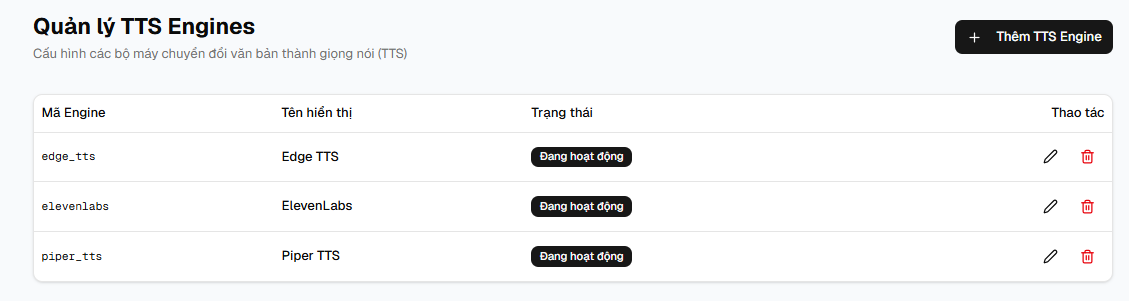
\includegraphics[width=0.92\textwidth]{images/WebUI-AdminEngines.png}
\caption{Quản lý engine}
\end{figure}

\textbf{Hướng dẫn:}

\begin{enumerate}
\item Admin mở trang cấu hình engine.
\item Kiểm tra trạng thái các engine đang hỗ trợ.
\item Bật, tắt hoặc cập nhật thông tin engine.
\end{enumerate}

\subsubsection{Quản lý giọng nói}

\begin{figure}[H]
\centering
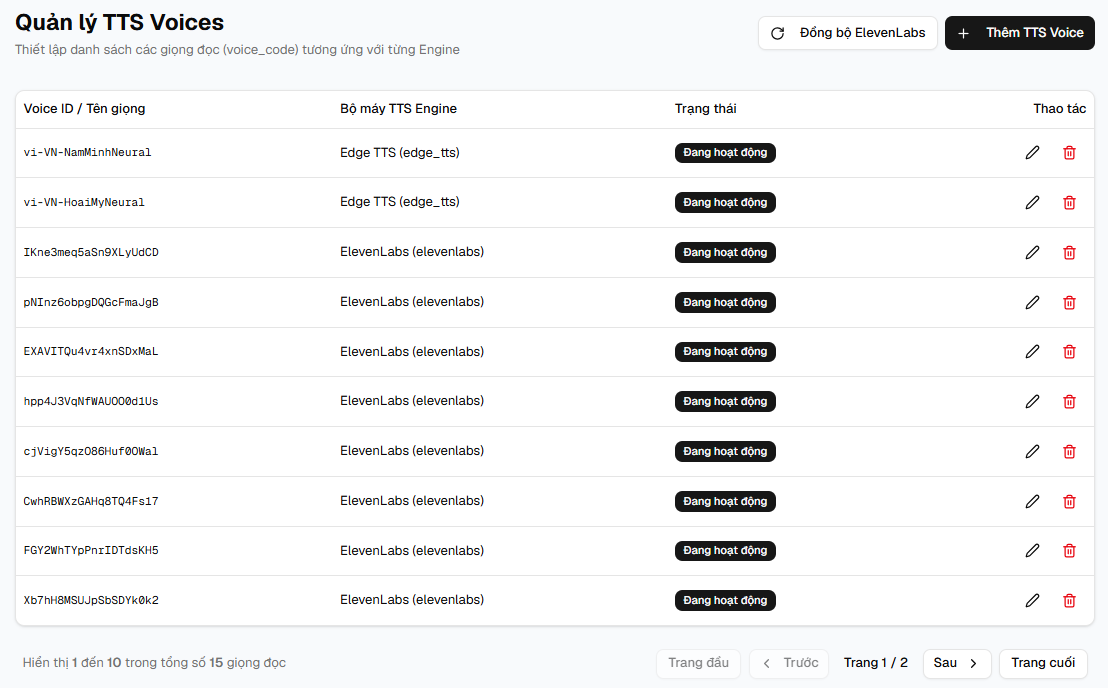
\includegraphics[width=0.92\textwidth]{images/WebUI-AdminVoices.png}
\caption{Quản lý giọng nói}
\end{figure}

\textbf{Hướng dẫn:}

\begin{enumerate}
\item Admin mở trang giọng nói.
\item Đồng bộ hoặc cập nhật danh sách voice.
\item Gắn voice phù hợp cho nhân vật AI.
\end{enumerate}

\subsubsection{Pipeline dữ liệu VBPL}

\begin{figure}[H]
\centering
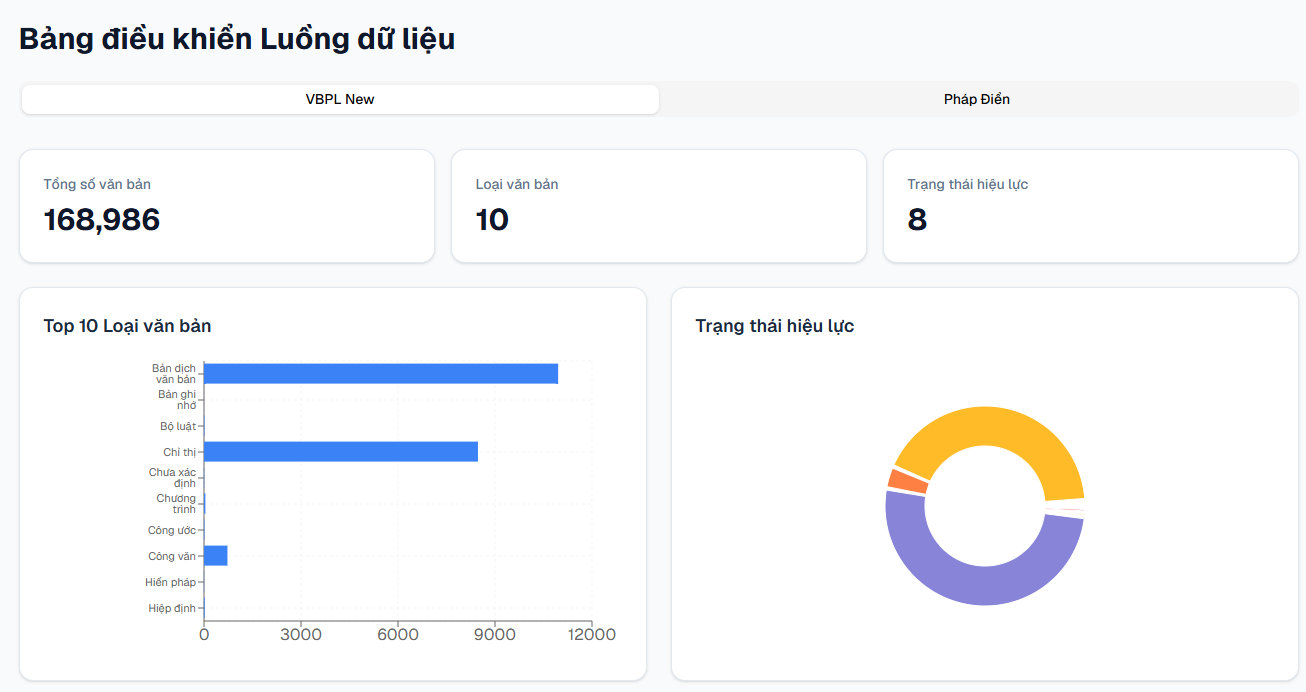
\includegraphics[width=0.92\textwidth]{images/WebUI-AdminDataPipelineVbpl.png}
\caption{Pipeline dữ liệu VBPL}
\end{figure}

\textbf{Hướng dẫn:}

\begin{enumerate}
\item Admin mở trang pipeline dữ liệu VBPL.
\item Theo dõi trạng thái xử lý dữ liệu.
\item Kiểm tra tiến độ hoặc lỗi nếu có.
\end{enumerate}

\subsubsection{Pipeline dữ liệu Pháp Điển}

\begin{figure}[H]
\centering
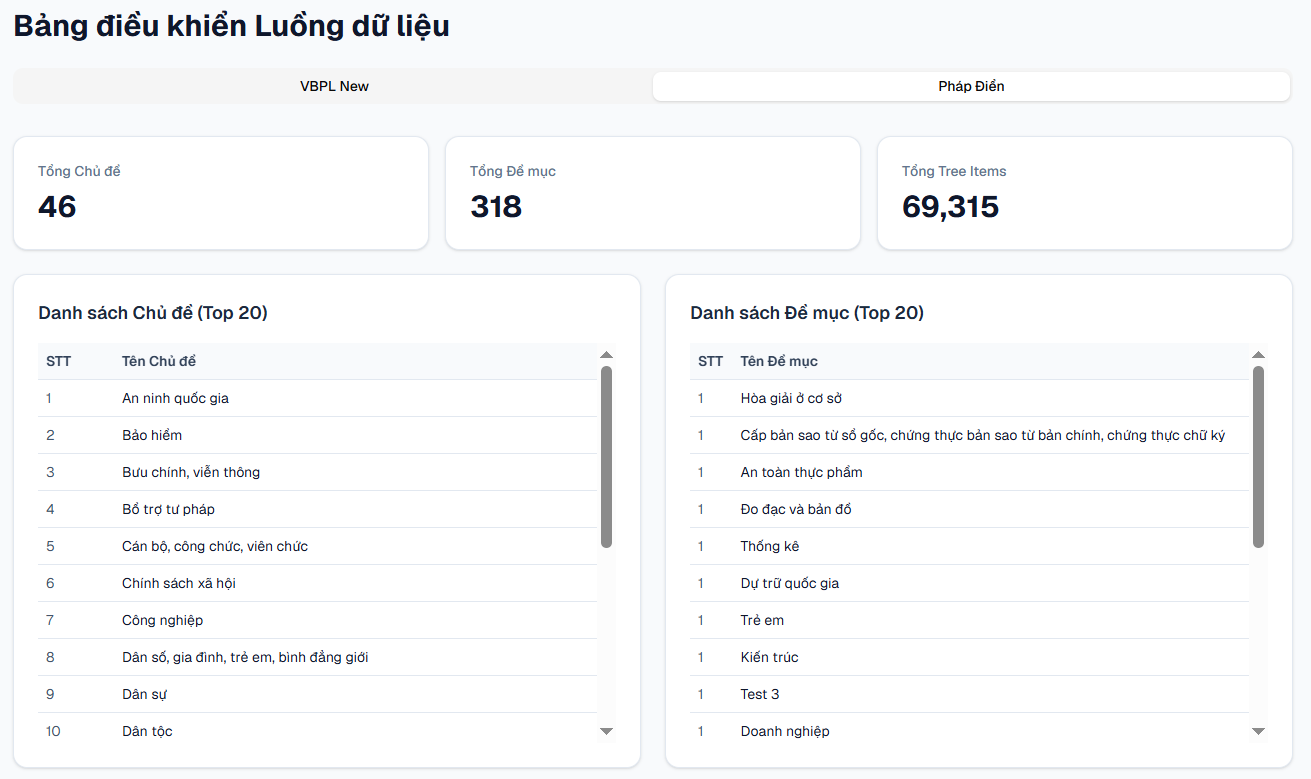
\includegraphics[width=0.92\textwidth]{images/WebUI-AdminDataPipelinePhapDien.png}
\caption{Pipeline dữ liệu Pháp Điển}
\end{figure}

\textbf{Hướng dẫn:}

\begin{enumerate}
\item Admin mở trang pipeline Pháp Điển.
\item Xem thống kê cấu trúc và tiến độ xử lý.
\item Dùng thông tin này để theo dõi chất lượng dữ liệu nền.
\end{enumerate}

\subsection{4. Thanh toán và gói VIP}

\subsubsection{Danh sách gói thanh toán}

\begin{figure}[H]
\centering
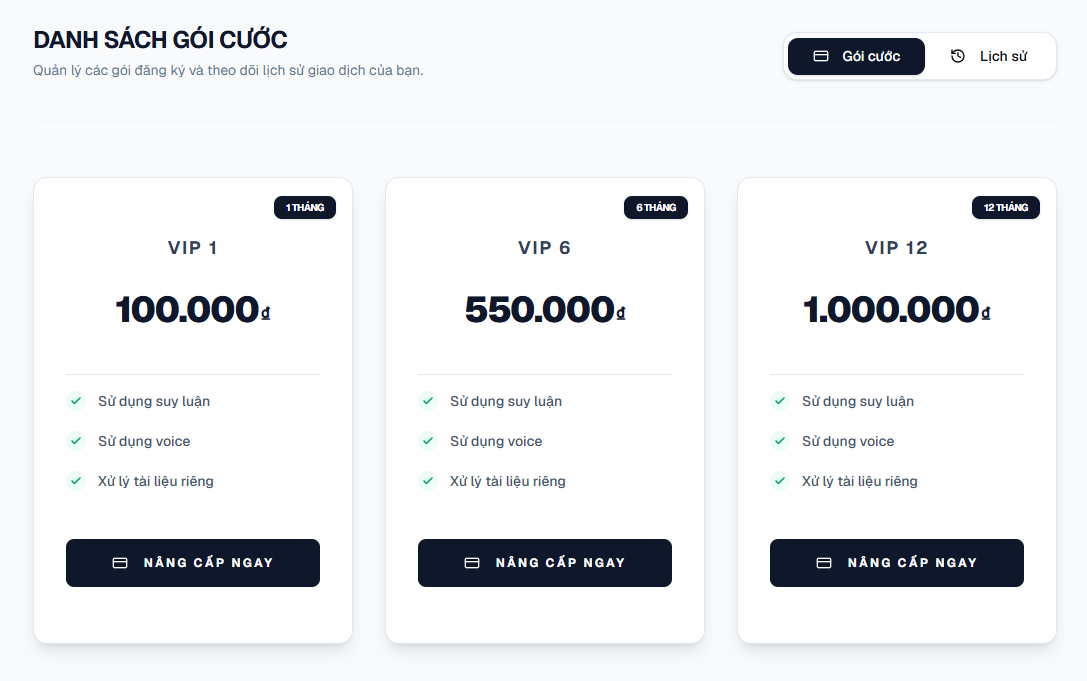
\includegraphics[width=0.92\textwidth]{images/WebUI-PaymentPlanList.png}
\caption{Danh sách gói thanh toán}
\end{figure}

\textbf{Hướng dẫn:}

\begin{enumerate}
\item Người dùng mở trang gói VIP.
\item So sánh quyền lợi, giá và thời hạn từng gói.
\item Chọn gói phù hợp để tiến hành thanh toán.
\end{enumerate}

\subsubsection{Lịch sử thanh toán}

\begin{figure}[H]
\centering
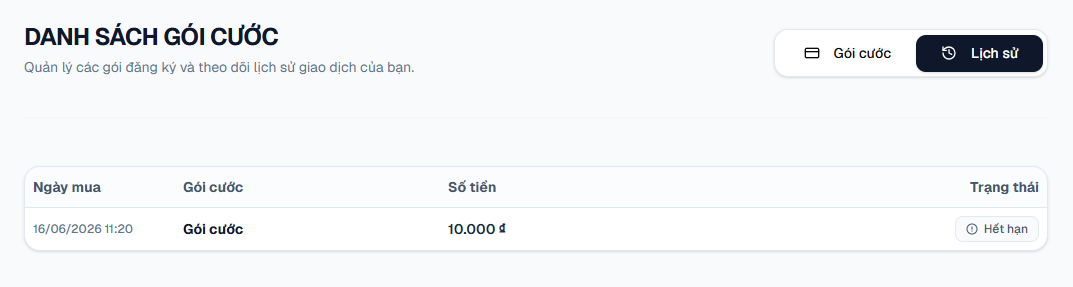
\includegraphics[width=0.92\textwidth]{images/WebUI-PaymentHistory.png}
\caption{Lịch sử thanh toán}
\end{figure}

\textbf{Hướng dẫn:}

\begin{enumerate}
\item Mở trang lịch sử giao dịch.
\item Kiểm tra trạng thái, thời gian và gói đã thanh toán.
\item Dùng thông tin này để đối soát giao dịch khi cần.
\end{enumerate}

\subsubsection{Thanh toán thành công}

\begin{figure}[H]
\centering
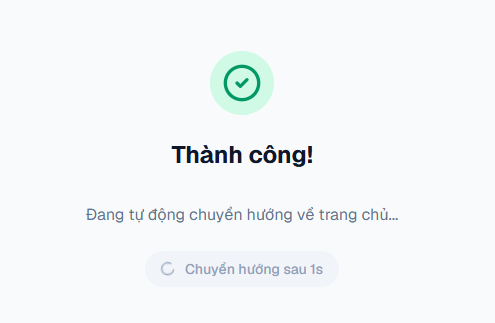
\includegraphics[width=0.92\textwidth]{images/WebUI-PaymentSuccess.png}
\caption{Thanh toán thành công}
\end{figure}

\textbf{Hướng dẫn:}

\begin{enumerate}
\item Sau khi thanh toán, hệ thống hiển thị kết quả thành công.
\item Kiểm tra thông tin gói VIP vừa kích hoạt.
\item Quay lại hệ thống để sử dụng các tính năng VIP.
\end{enumerate}

\subsubsection{Email thanh toán thành công}

\begin{figure}[H]
\centering
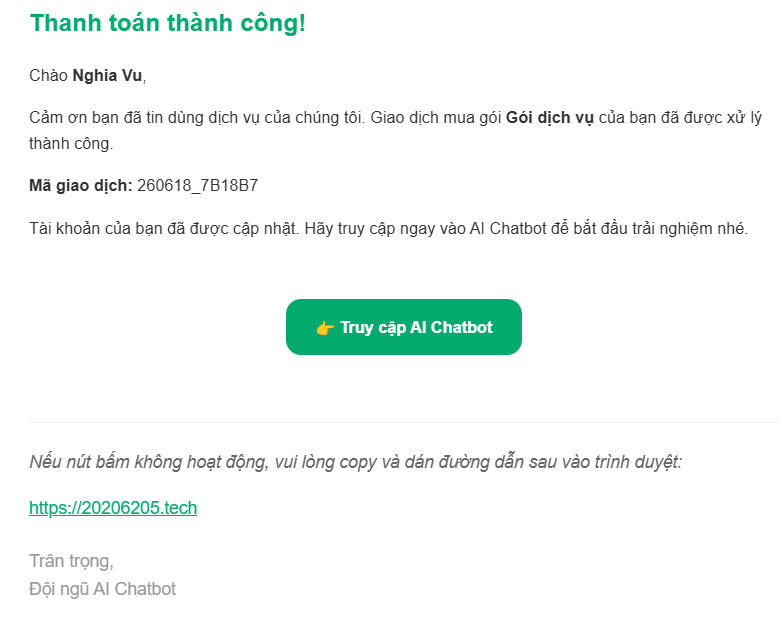
\includegraphics[width=0.92\textwidth]{images/WebUI-PaymentSuccessEmail.png}
\caption{Email thanh toán thành công}
\end{figure}

\textbf{Hướng dẫn:}

\begin{enumerate}
\item Mở email thông báo thanh toán.
\item Kiểm tra thông tin gói, thời hạn và trạng thái giao dịch.
\item Lưu email để đối chiếu khi cần hỗ trợ.
\end{enumerate}

\subsubsection{Gói VIP đang hoạt động}

\begin{figure}[H]
\centering
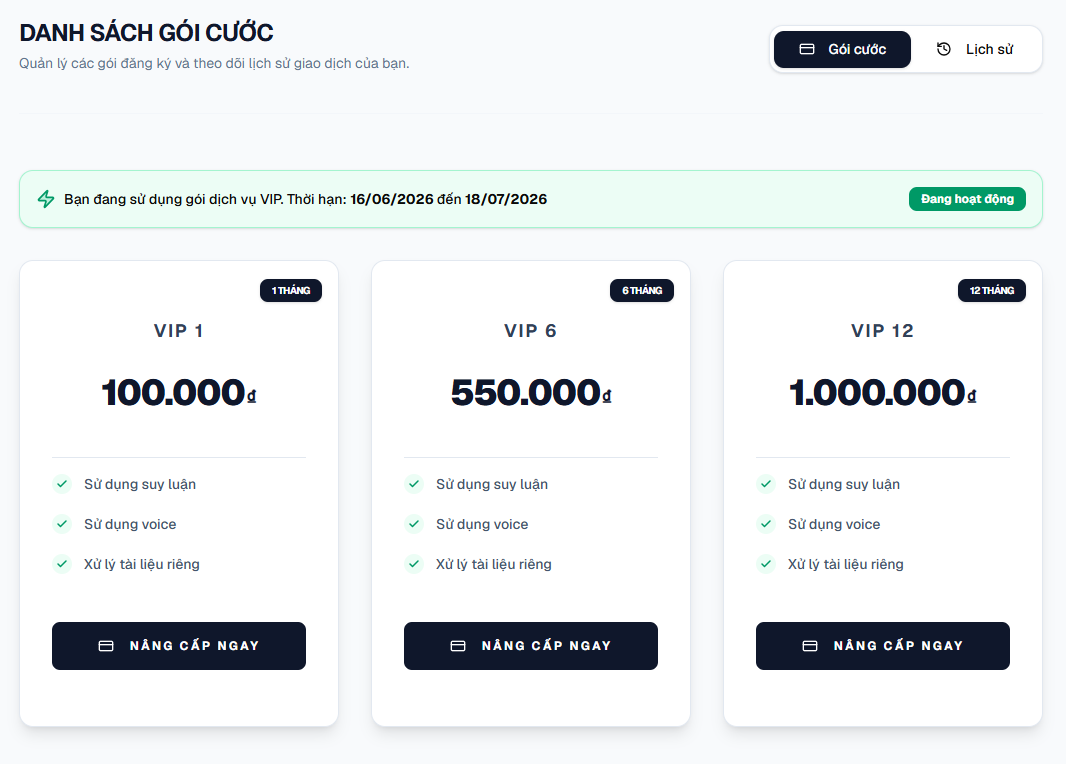
\includegraphics[width=0.92\textwidth]{images/WebUI-PaymentPlanActive.png}
\caption{Gói VIP đang hoạt động}
\end{figure}

\textbf{Hướng dẫn:}

\begin{enumerate}
\item Mở trang gói VIP sau khi thanh toán.
\item Kiểm tra dấu hiệu gói đang hoạt động.
\item Sử dụng các tính năng yêu cầu VIP như reasoning, voice chat hoặc tài liệu cá nhân.
\end{enumerate}

\subsection{5. Voice chat}

\subsubsection{Chọn giọng nói}

\begin{figure}[H]
\centering
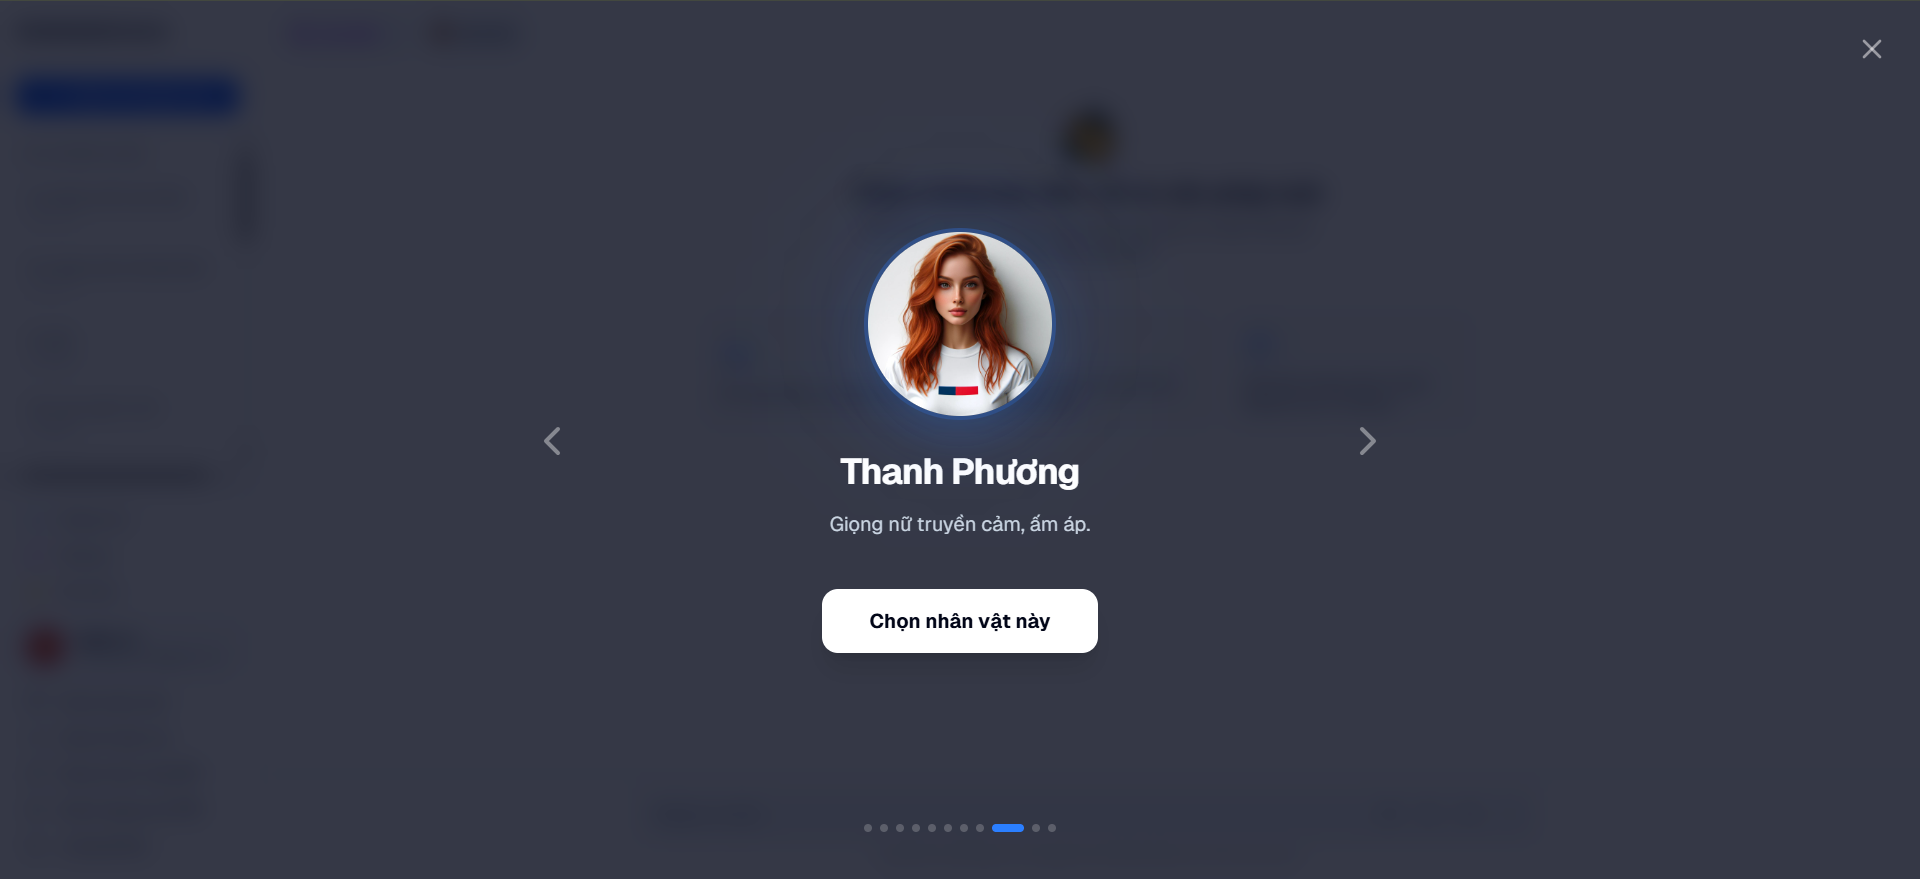
\includegraphics[width=0.92\textwidth]{images/WebUI-VoiceSelect.png}
\caption{Chọn giọng nói}
\end{figure}

\textbf{Hướng dẫn:}

\begin{enumerate}
\item Mở phần chọn giọng nói hoặc nhân vật.
\item Nghe thử hoặc xem thông tin từng giọng.
\item Chọn giọng phù hợp cho phiên trò chuyện.
\end{enumerate}

\subsubsection{Trò chuyện bằng giọng nói}

\begin{figure}[H]
\centering
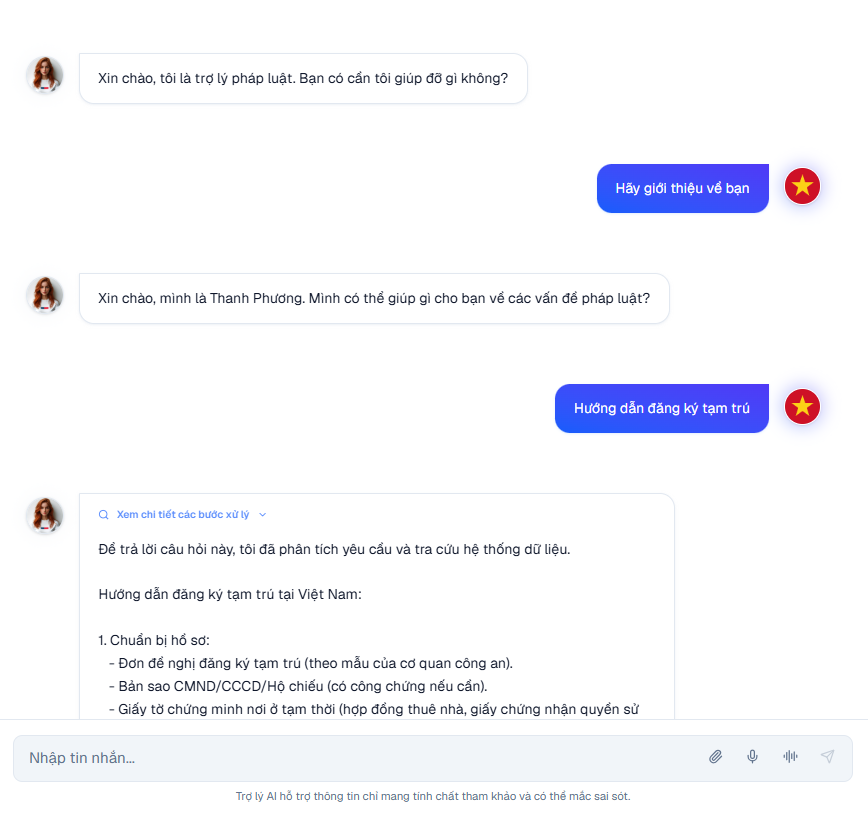
\includegraphics[width=0.92\textwidth]{images/WebUI-VoiceChat.png}
\caption{Trò chuyện bằng giọng nói}
\end{figure}

\textbf{Hướng dẫn:}

\begin{enumerate}
\item Bắt đầu phiên voice chat.
\item Nói câu hỏi hoặc yêu cầu vào micro.
\item Nghe phản hồi bằng giọng nói và theo dõi trạng thái xử lý trên giao diện.
\end{enumerate}

\subsection{6. Tài liệu cá nhân}

\subsubsection{Tải lên tài liệu}

\begin{figure}[H]
\centering
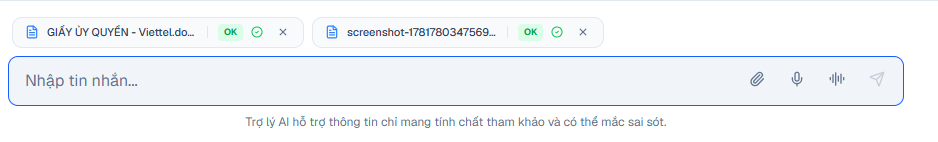
\includegraphics[width=0.92\textwidth]{images/WebUI-DocumentUpload.png}
\caption{Tải lên tài liệu}
\end{figure}

\textbf{Hướng dẫn:}

\begin{enumerate}
\item Chọn file tài liệu từ thiết bị.
\item Bấm tải lên.
\item Chờ hệ thống xử lý nền trước khi dùng tài liệu trong chat.
\end{enumerate}

\subsubsection{Chat với tài liệu}

\begin{figure}[H]
\centering
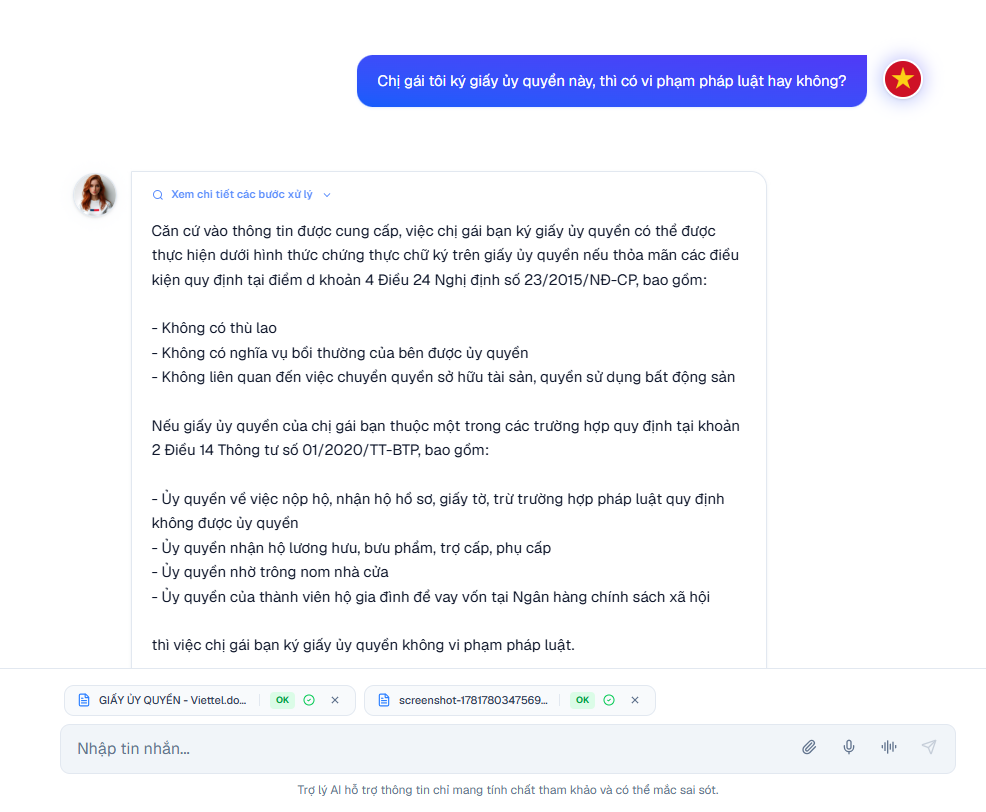
\includegraphics[width=0.92\textwidth]{images/WebUI-DocumentChat.png}
\caption{Chat với tài liệu}
\end{figure}

\textbf{Hướng dẫn:}

\begin{enumerate}
\item Chọn tài liệu đã xử lý thành công.
\item Đặt câu hỏi liên quan đến nội dung tài liệu.
\item Xem câu trả lời và nguồn tham chiếu do hệ thống trả về.
\end{enumerate}
